% !TEX encoding = UTF-8 Unicode
\documentclass[]{article}
\errorcontextlines 1000000
% we want a left aligned text not centered
\usepackage{ragged2e}
% needed for pandoc table generation
\usepackage{longtable, booktabs, array, calc}
% This takes care of quotes and all that
\usepackage[autostyle=true,german=quotes]{csquotes}
\usepackage{floatrow}
\floatsetup[figure]{capposition=top}
% actually not needed
% also I found the beamer stuff pretty ugly
% % the next one I need to explore more
% how to set the fonts right
% lots of packages that I don't know
\usepackage{lmodern}

\usepackage{setspace}


\usepackage{amssymb,amsmath}
\usepackage{ifxetex,ifluatex}
\usepackage{fixltx2e} % provides \textsubscript
\ifnum 0\ifxetex 1\fi\ifluatex 1\fi=0 % if pdftex
  \usepackage[T1]{fontenc}
  \usepackage[utf8]{inputenc}
\else % if luatex or xelatex
  \ifxetex
    \usepackage{mathspec}
  \else
    \usepackage{fontspec}
  \fi
  \defaultfontfeatures{Ligatures=TeX,Scale=MatchLowercase}
% yes it is on euro
% does that mean I can use the \euro command to
% get an €? How inconvinient
% more font options
% the problem is I tried these but did not change the font
\fi
% use upquote if available, for straight quotes in verbatim environments
\IfFileExists{upquote.sty}{\usepackage{upquote}}{}
% use microtype if available
\IfFileExists{microtype.sty}{%
\usepackage[]{microtype}
\UseMicrotypeSet[protrusion]{basicmath} % disable protrusion for tt fonts
}{}
\PassOptionsToPackage{hyphens}{url} % url is loaded by hyperref

% another option to investigate
%
\usepackage[unicode=true]{hyperref}
% so why is my subtitle and all that not set?
\hypersetup{
            pdfborder={0 0 0},
            breaklinks=true}
\urlstyle{same}  % don't use monospace font for urls

% change the margins of the page
% I might do that later
% language support
% you need to use language codes de-DE or de-AT
\usepackage{graphicx,grffile}
\makeatletter
\def\maxwidth{\ifdim\Gin@nat@width>\linewidth\linewidth\else\Gin@nat@width\fi}
\def\maxheight{\ifdim\Gin@nat@height>\textheight\textheight\else\Gin@nat@height\fi}
\makeatother
% Scale images if necessary, so that they will not overflow the page
% margins by default, and it is still possible to overwrite the defaults
% using explicit options in \includegraphics[width, height, ...]{}
\setkeys{Gin}{width=\maxwidth,height=\maxheight,keepaspectratio}
% so we can push the links into footnotes?
% nice
\IfFileExists{parskip.sty}{%
\usepackage{parskip}
}{% else
\setlength{\parindent}{0pt}
\setlength{\parskip}{6pt plus 2pt minus 1pt}
}
\setlength{\emergencystretch}{3em}  % prevent overfull lines
\providecommand{\tightlist}{%
  \setlength{\itemsep}{0pt}\setlength{\parskip}{0pt}}
\setcounter{secnumdepth}{0}
% Redefines (sub)paragraphs to behave more like sections
\ifx\paragraph\undefined\else
\let\oldparagraph\paragraph
\renewcommand{\paragraph}[1]{\oldparagraph{#1}\mbox{}}
\fi
\ifx\subparagraph\undefined\else
\let\oldsubparagraph\subparagraph
\renewcommand{\subparagraph}[1]{\oldsubparagraph{#1}\mbox{}}
\fi

% set default figure placement to htbp
% https://tex.stackexchange.com/a/2282/133290
% added the !
\makeatletter
\def\fps@figure{!htbp}
\makeatother


\date{}
\begin{document}
\RaggedRight

\newpage
{
\setcounter{tocdepth}{3}
\tableofcontents
}
\newpage
\hypertarget{einleitung}{%
\section{Einleitung}\label{einleitung}}

\begin{figure}
\hypertarget{fig:splash}{%
\centering

\includegraphics{assets/images/splash.png}
\caption{Offizieller (und ultimative) Splash Screen}\label{fig:splash}
}
\end{figure}

Dieses Dokument ist der Versuch, den gesamten Prozess der Bedienung der
Laser Anlage an der Fachhochschule Potsdam zu dokumentieren. Es sollte
aufmerksam gelesen werden, bevor die Anlage durch Studierende in betrieb
genommen wird. Am Ende des Dokuments befindet sich eine
\protect\hyperlink{checklist}{Checkliste}, die ausgedruckt und als
Spickzettel beim Betrieb verwendet werden kann. In einigen Bereichen wie
der Aufbereitung von Daten und der Bedienung der Software geht es nicht
in die Tiefe. Wir hoffen, dass dies als ein "lebendes" Dokument genutzt
wird und zukünftig, um nützliche Bereiche erweitert wird. Anregungen,
Fragen, Fehler können auf
\href{https://github.com/FH-Potsdam/the-ultimate-laser-guide/issues}{GitHub
als Issue} vorgebracht werden oder per Mail an die Autoren gesendet
werden. Das Dokument selber kann als PDF
\href{https://github.com/FH-Potsdam/the-ultimate-laser-guide/raw/master/The-Ultimate-Laser-Guide.pdf}{hier}
runtergeladen werden. Eine HTML-Version ist
\href{https://fh-potsdam.github.io/the-ultimate-laser-guide/}{hier} zu
finden. Wir freuen uns über jede Art von Beitrag. Gerne nehmen wir auch
weitere Kapitel an (siehe Abschnitt
\protect\hyperlink{uxfcber-dieses-dokument}{Über dieses Dokument})

Viel Spaß mit dem "Ultimativen Laser Handbuch"\footnote{Ultimative ist
  vielleicht ein wenig übertrieben.}!

\hypertarget{grundlegende-voraussetzungen-sind...}{%
\subsection{Grundlegende Voraussetzungen
sind...}\label{grundlegende-voraussetzungen-sind...}}

\begin{itemize}
\tightlist
\item
  Die Unterzeichnung und Anerkennung der Werkstattordnung.
\item
  Die Teilnahme an der Sicherheitseinweisung durch Anne Boenisch und
  oder eine Freigabe durch sie.
\item
  Der Laser wird immer in Gruppen von 2 oder mehr Personen betrieben.\\
\item
  Der Laser wird nicht alleine gelassen, während er läuft.\\
\item
  Die Werkstatt wird nach Nutzung wieder aufgeräumt.\\
\item
  Der Laser wird nach Gebrauch gereinigt.\\
\item
  Es dürfen \textbf{KEINE} PVC-haltigen oder leicht entflammbare
  Materialien geschnitten werden (siehe Abschnitt
  \protect\hyperlink{materialien}{Materialien}).
\end{itemize}

\hypertarget{sicherheit}{%
\subsection{Sicherheit}\label{sicherheit}}

Die Anlage darf nicht alleine betrieben werden. Es müssen immer
mindestens 2 Personen vor Ort sein.

\hypertarget{feuer}{%
\subsubsection{Feuer?}\label{feuer}}

Im Falle eines Feuers in der Anlage gilt es Ruhe zu bewahren. Folgende
Schritte sind auszuführen.

\begin{enumerate}
\def\labelenumi{\arabic{enumi}.}
\tightlist
\item
  Laservorgang stoppen! (Notaus oder \texttt{Start/Stop} Knopf)
\item
  Lüftung abschalten!
\item
  CO2 Feuerlöscher benutzen! (Falls es immer noch brennen sollte)
\item
  Die Feuerwehr rufen, wenn der Brand nicht zu löschen ist!
\end{enumerate}

\textbf{Hinweise:}

\begin{itemize}
\tightlist
\item
  Es sollte bis zum Einsatz des Feuerlöscher die Abdeckung nicht
  geöffnet werden.\\
\item
  Es sollten niemals Flüssigkeiten verwendet werden, um den Brand zu
  löschen.
\end{itemize}

\hypertarget{notaus}{%
\subsubsection{Notaus?}\label{notaus}}

Der Notaus (siehe +@fig:steuerung) ist für den Notfall. Wenn dieser
gedrückt wurde, sollte genau überlegt werden, ob die Anlage wieder in
Betrieb genommen werden kann, ohne sie zu beschädigen. Im Zweifelsfalle
sind die Administratoren zu kontaktieren. Wenn der Notaus gedrückt wurde
und wieder raus gezogen wird, startet die gesamte Anlage neu.\footnote{Um
  die sofortige Referenzfahrt zu verhindern, sollte der Schlüssel im
  \texttt{An/Aus} Schlüsselloch auf Aus gedreht werden (siehe
  +@fig:steuerung).} Der Laserkopf führt eine Referenzfahrt aus. Es gilt
vorab darauf zu achten, dass der Kopf bei dieser Fahrt nicht beschädigt
wird.

\hypertarget{pflege-der-anlage}{%
\subsection{Pflege der Anlage}\label{pflege-der-anlage}}

\begin{quote}
Eine verschmutzte Maschine ist bald eine defekte Maschine.\\
-- Fabian Morón Zirfas
\end{quote}

Damit der Laser lange betrieben werden kann, muss er regelmäßig
gereinigt werden. Dies passiert durch die Studierenden. Sie sind selber
dazu angehalten dies zu organisieren. Nach jedem Gebrauch muss der
Innenraum der Anlage ausgesaugt werden und etwaige Reste müssen entfernt
werden. Ebenfalls muss der Taster gereinigt werden. Die Reinigung wird
nur bei ausgeschalteter Anlage durchgeführt.

In der Metallwerkstatt stehen hinter der Tür zwei Kisten. In der einen
gibt es saubere Tücher. Diese dürfen verwendet werden, um den Laser
sauber zu machen.

\hypertarget{wechseln-der-filter}{%
\subsubsection{Wechseln der Filter}\label{wechseln-der-filter}}

to be defined\ldots{}

\hypertarget{reinigung-der-spiegel}{%
\subsubsection{Reinigung der Spiegel}\label{reinigung-der-spiegel}}

\begin{figure}
\hypertarget{fig:spiegel}{%
\centering
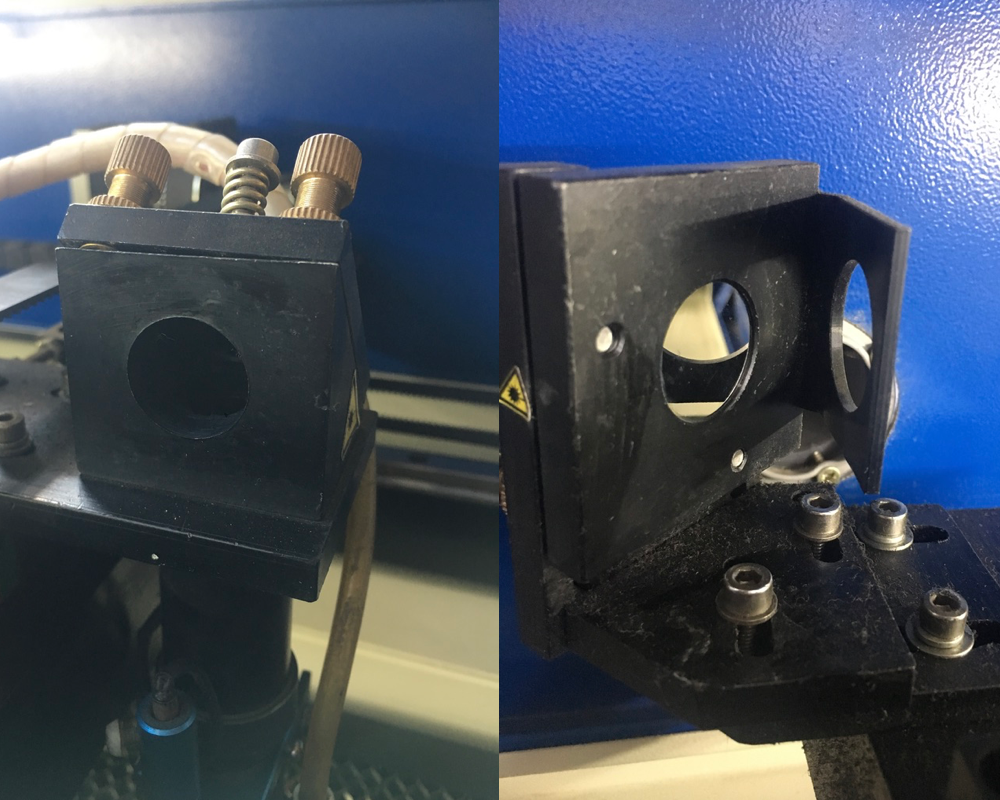
\includegraphics{assets/images/laser-spiegel.png}
\caption{Die Spiegel}\label{fig:spiegel}
}
\end{figure}

Zur Reinigung der Spiegel (siehe +@fig:spiegel) darf nur Isopropanol und
Q-Tip verwendet werden. Dies sollte mindestens einmal im Monat
durchgeführt werden, um eine konstante Leistung des Lasers zu
garantieren.

\hypertarget{reinigung-der-sichtscheiben}{%
\subsubsection{Reinigung der
Sichtscheiben}\label{reinigung-der-sichtscheiben}}

Zur Reinigung der Sichtscheiben darf kein alkoholhaltiges Mittel
benutzen werden. Normale Lappen oder Papiertücher zerkratzen die Scheibe
schnell und stark. Die Scheibe ist aus PolyCarbonat und kann somit auch
nicht so leicht wieder aufpoliert werden wie zum Beispiel Acrylglas.
Daher sollten zur Reiniung nur mit Wasser befeuchtete Microfasertücher
genutzt werden.

\hypertarget{reinigung-des-arbeitsraums}{%
\subsubsection{Reinigung des
Arbeitsraums}\label{reinigung-des-arbeitsraums}}

\begin{figure}
\hypertarget{fig:saugmobil}{%
\centering
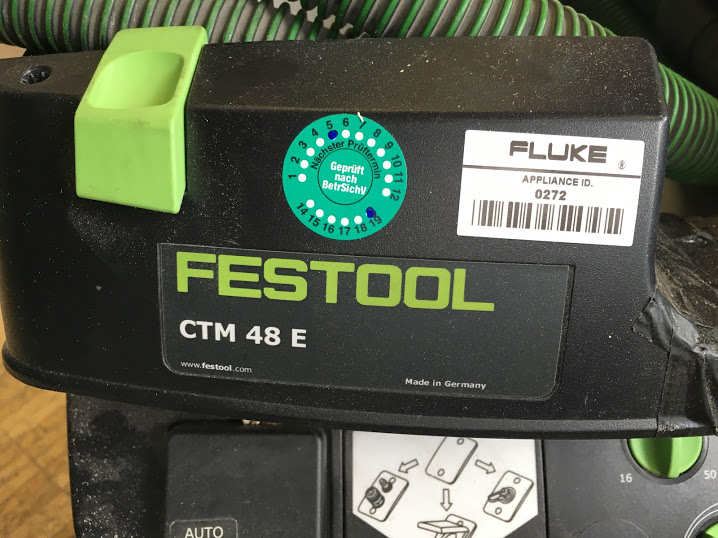
\includegraphics{assets/images/festo-saugmobil.jpg}
\caption{Das Festo CTM 48 E Saugmobil}\label{fig:saugmobil}
}
\end{figure}

Der Arbeitsraum und auch die unteren Bereiche der Anlage müssen
regelmäßig gereinigt werden. Für eine oberflächliche Reinigung kann das
"Festo CTM 48 E Saugmobil" der Modellbauwerkstatt genutzt werden, um die
Anlage auszusaugen (siehe +@fig:saugmobil). Es sollte jedoch auch
regelmäßig mit einem Lappen eine tiefer gehende Reinigung vorgenommen
werden. Auch unterhalb des Gitters und der Lamellen sowie im unteren
Raum des Lasers.\footnote{Zum öffnen der äußeren Verkleidung gibt es in
  der Werkzeugkiste Dreikantschlüssel.}

\hypertarget{reinigung-des-distanztasters}{%
\subsubsection{Reinigung des
Distanztasters}\label{reinigung-des-distanztasters}}

Vor jedem Gebrach muss überprüft werden, ob der Taster sich bewegen
lässt. Nach jedem Gebrauch sollte der Taster mit einem Papiertuch von
Ruß befreit werden.

\hypertarget{reinigung-des-gitters}{%
\subsubsection{Reinigung des Gitters}\label{reinigung-des-gitters}}

Das Gitter, dass im Arbeitsraum der Anlage liegt, sollte regelmäßig
gereinigt werden. Wenn es zu sehr verschmutzt ist, werden Rußreste, die
auf dem Gitter sind, durch den Laser nochmals entzündet. Diese
schmauchen auf die Unterseite des Materials und hinterlassen unschöne
Spuren. Daher ist es auch Sinne der Studierenden die Reinigung
regelmäßig durchzuführen, um bestmögliche Ergebnisse zu erzielen.

Um das Gitter zu reinigen sollte, die Wanne der Siebdruckwerkstatt und
deren Kärcher genutzt werden.\footnote{Die Erlaubnis der
  Siebdruckwerkstatt muss vorher eingeholt werden.}

\hypertarget{entsorgung-der-schnittreste}{%
\subsubsection{Entsorgung der
Schnittreste}\label{entsorgung-der-schnittreste}}

\begin{figure}
\hypertarget{fig:schnitt-reste}{%
\centering
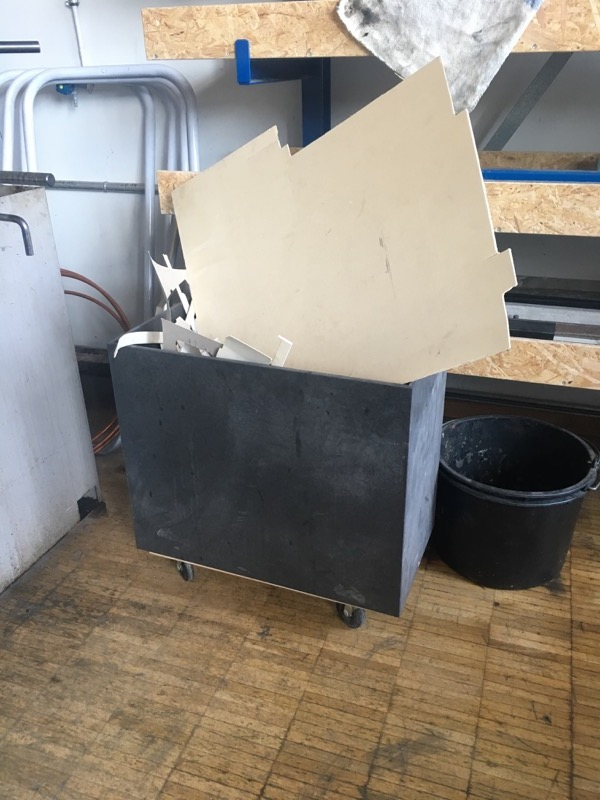
\includegraphics{assets/images/laser-schnittreste.JPG}
\caption{Der Rollkorb für Schnittreste}\label{fig:schnitt-reste}
}
\end{figure}

Für Schnittreste existiert ein eigener Abfallbehälter (siehe
+@fig:schnitt-reste). Dieser muss selbständig und regelmäßig entleert
werden.

\hypertarget{inbetriebnahme}{%
\subsection{Inbetriebnahme}\label{inbetriebnahme}}

Die folgenden Punkte \textbf{müssen} in der angegebenen Reihenfolge
ausgeführt werden. \emph{Die \protect\hyperlink{checklist}{Checkliste}
sollte von ungeübten Nutzer/innen zu Rate gezogen werden.}

\hypertarget{oberlicht-uxf6ffnen}{%
\subsubsection{Oberlicht Öffnen}\label{oberlicht-uxf6ffnen}}

\begin{figure}
\hypertarget{fig:oberlicht}{%
\centering
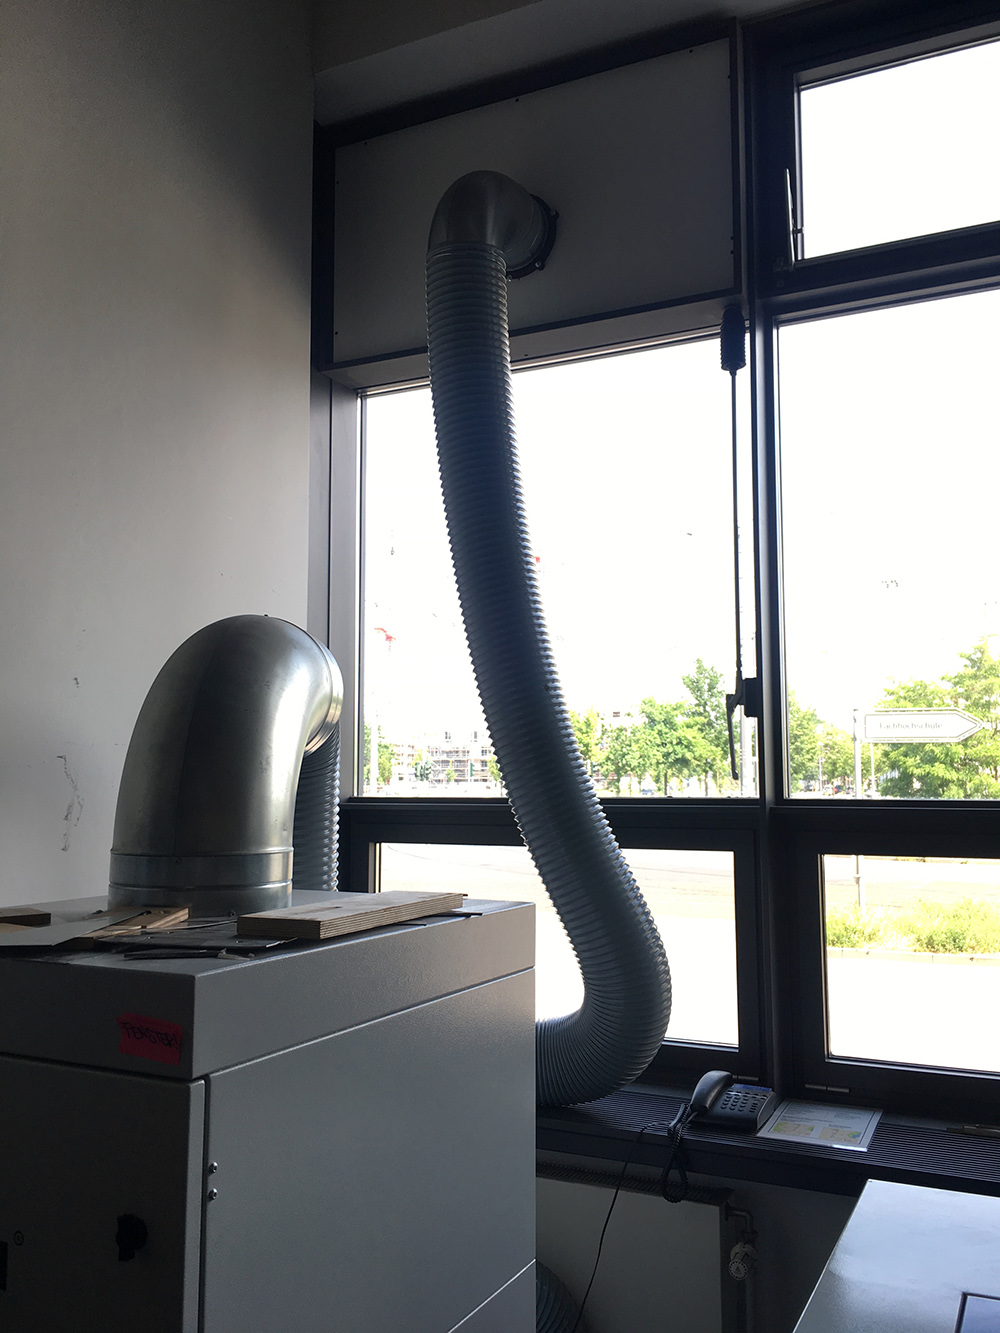
\includegraphics{assets/images/oberlicht.jpg}
\caption{Das Oberlicht des Lüfters}\label{fig:oberlicht}
}
\end{figure}

Damit eine arbeitsgerechte Abluft stattfinden kann, muss das Oberlicht
an das die Lüftung angeschlossen ist, geöffnet werden (siehe
+@fig:oberlicht).

\hypertarget{luxfcftung-einschalten}{%
\subsubsection{Lüftung Einschalten}\label{luxfcftung-einschalten}}

\begin{figure}
\hypertarget{fig:luefter}{%
\centering
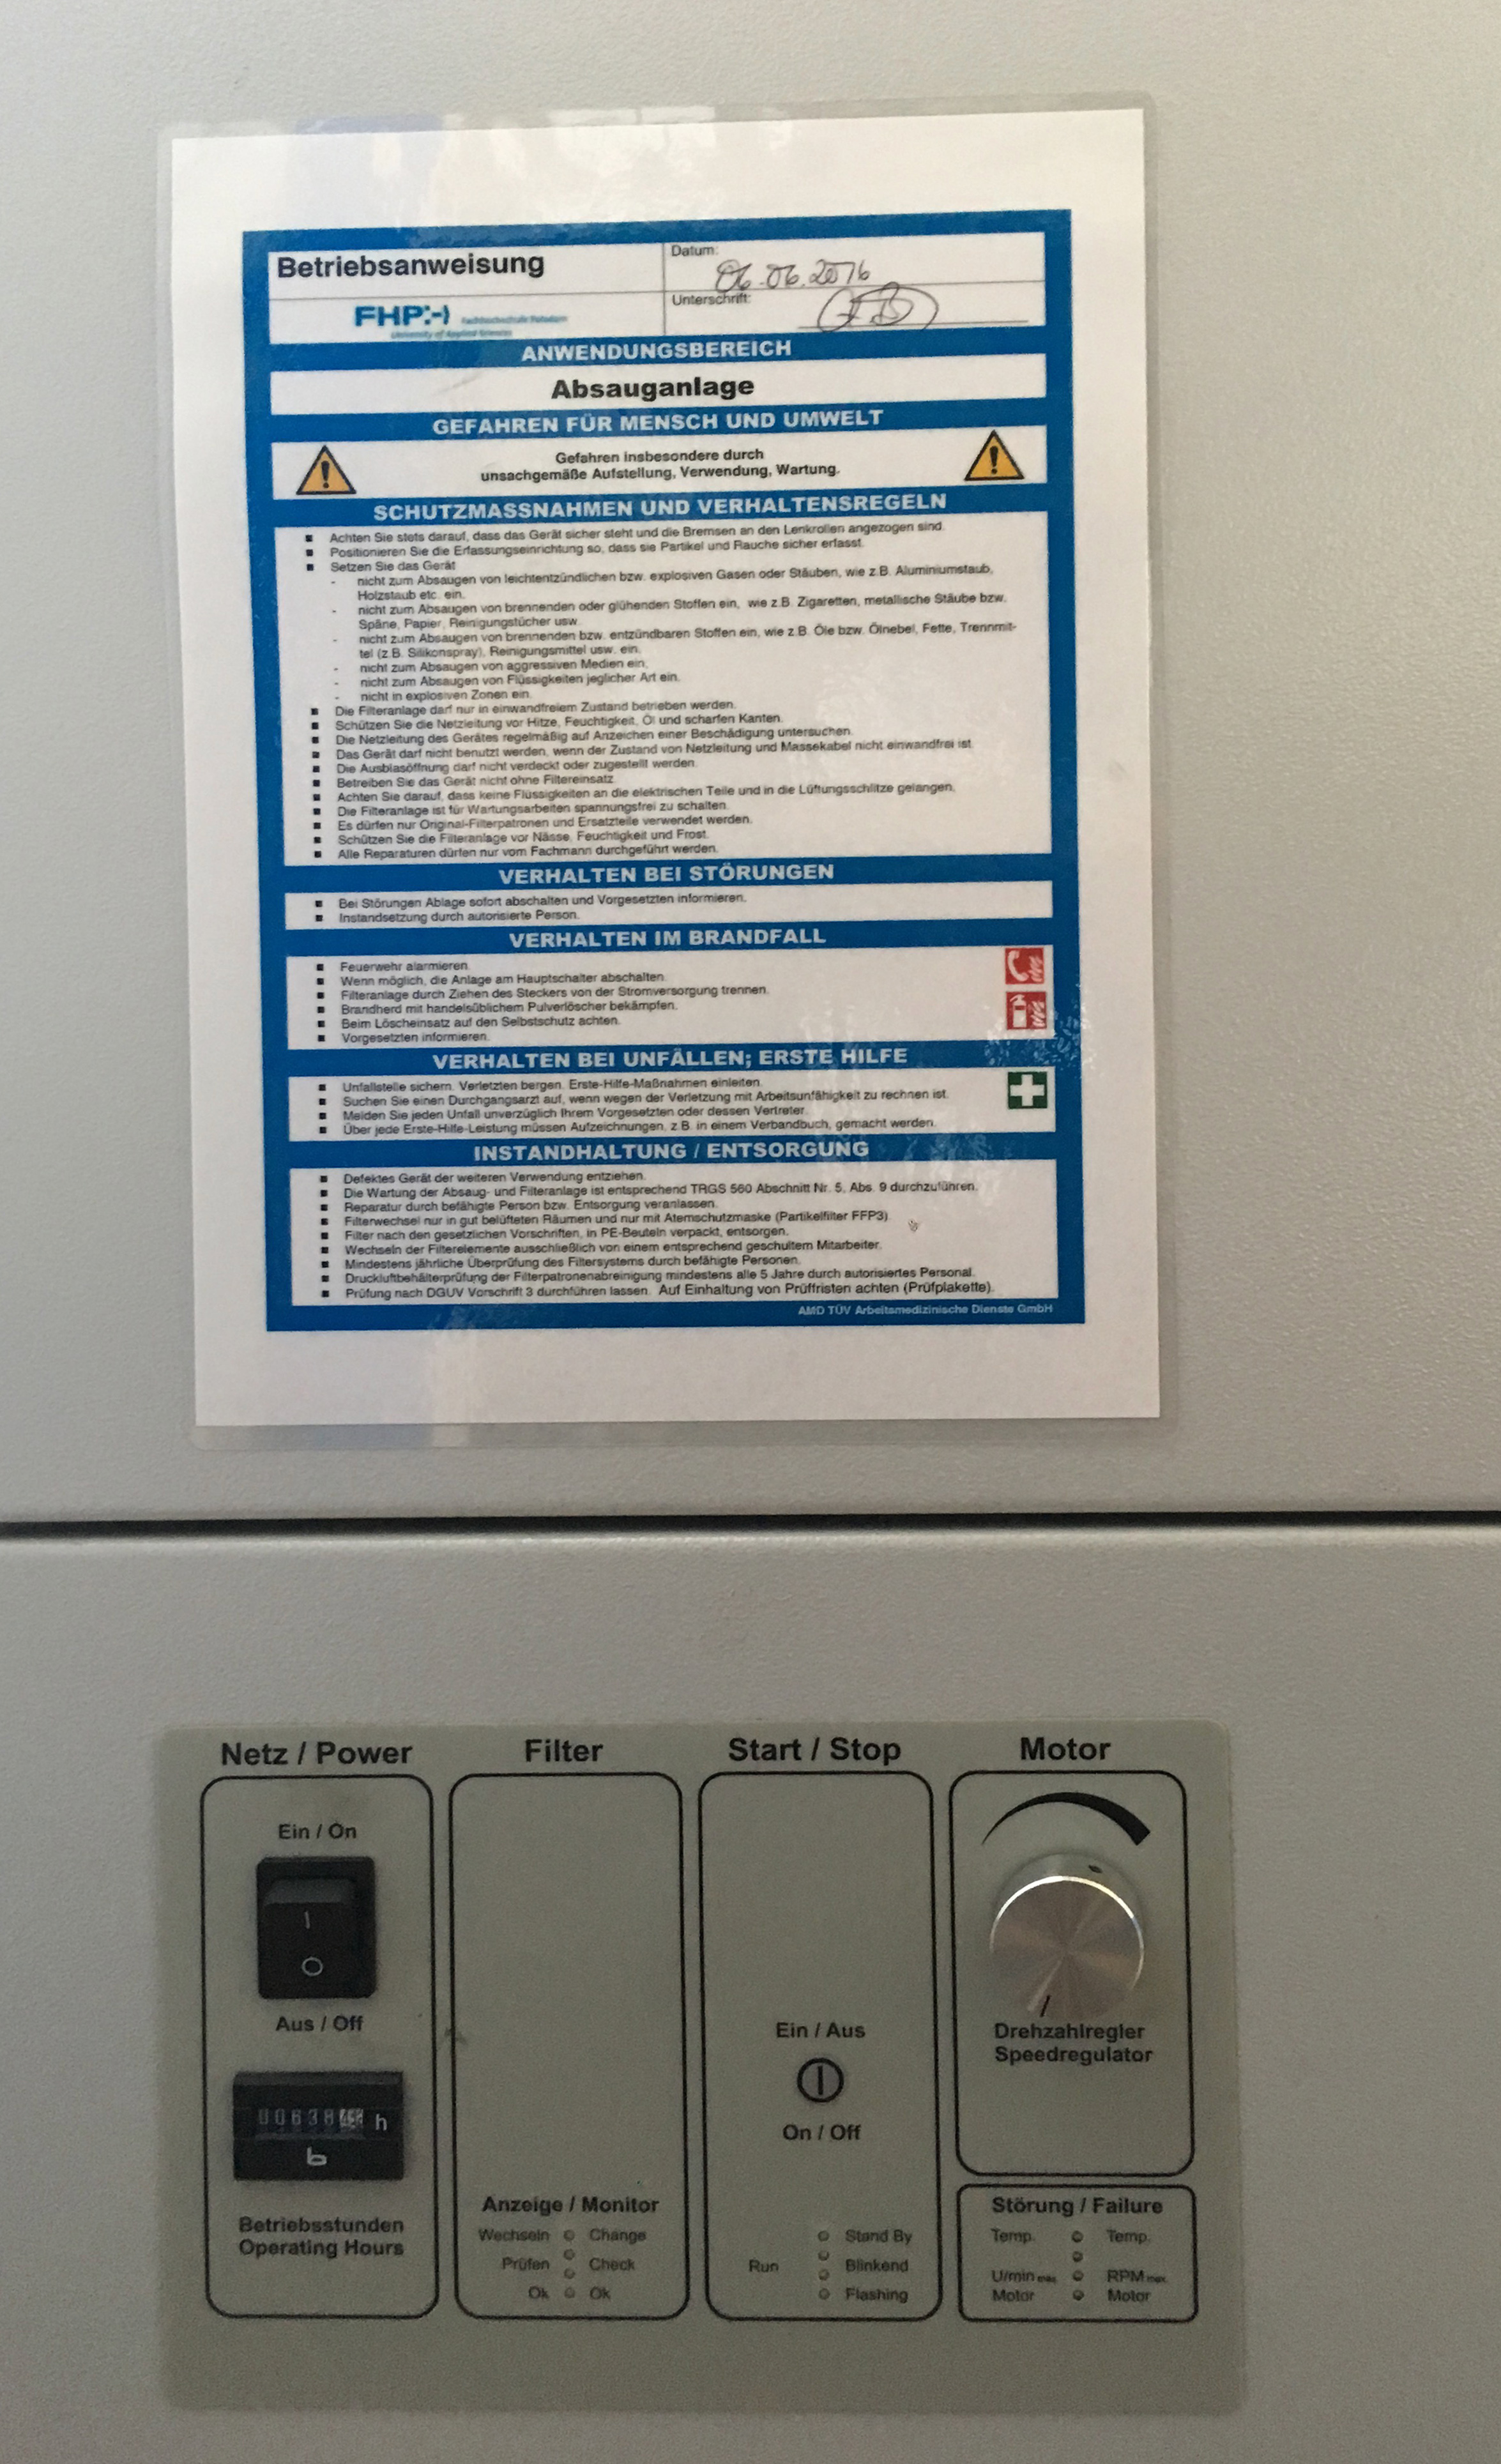
\includegraphics[width=0.5\textwidth,height=\textheight]{./assets/images/lueftung-steuerung.jpg}
\caption{Lüfter Steuerung}\label{fig:luefter}
}
\end{figure}

An der Lüftung gibt es den 4 Steuerungsbereiche (siehe +@fig:luefter).

\begin{enumerate}
\def\labelenumi{\arabic{enumi}.}
\tightlist
\item
  Netz/Power
\item
  Filter
\item
  Start/Stop
\item
  Motor
\end{enumerate}

Über den Hauptschalter in Bereich 1 wird die Lüftung aktiviert. Wenn im
Bereich 2 die Status-LED OK (grün) anzeigt, kann die Maschine in Betrieb
genommen werden. Steht sie auf Prüfen oder Wechseln müssen zuallererst
die zuständigen Personen kontaktiert werden. Die Anlage wird bis dahin
\textbf{nicht} in Betrieb genommen.

Über den \texttt{Start/Stop} Knopf in Bereich 3 kann die Lüftung
pausiert werden.

In Bereich 4 kann die Stärke der Lüftung angepasst werden. Der Lüfter
ist immer auf Stufe 4 zu nutzen. Gegen den dadurch entstehenden hohen
Geräuschpegel gibt es Hörschutz.

\hypertarget{arbeitsfluxe4che-leeren}{%
\subsubsection{Arbeitsfläche leeren}\label{arbeitsfluxe4che-leeren}}

Damit der Laserkopf bei der ersten Referenzfahrt in die rechte Obere
Ecke nicht beschädigt wird, darf kein Material bei der Inbetriebnahme
auf der Arbeitsfläche liegen.

\hypertarget{gitter-uxfcberpruxfcfen}{%
\subsubsection{Gitter Überprüfen}\label{gitter-uxfcberpruxfcfen}}

Das Gitter, dass in der Maschine liegt ist frei beweglich. Es muss vor
der Inbetriebnahme sichergestellt werden, dass es nicht unter die
Absätze links und rechts rutschen kann. Bei einem Autofokus oder fahren
der Z-Achse könnte sonst die Ausrichtung der Plattform beschädigt
werden. Diese muss dann manuell wieder in Waage gebracht werden.

\hypertarget{hauptstrom}{%
\subsubsection{Hauptstrom}\label{hauptstrom}}

\begin{figure}
\hypertarget{fig:hauptschalter}{%
\centering
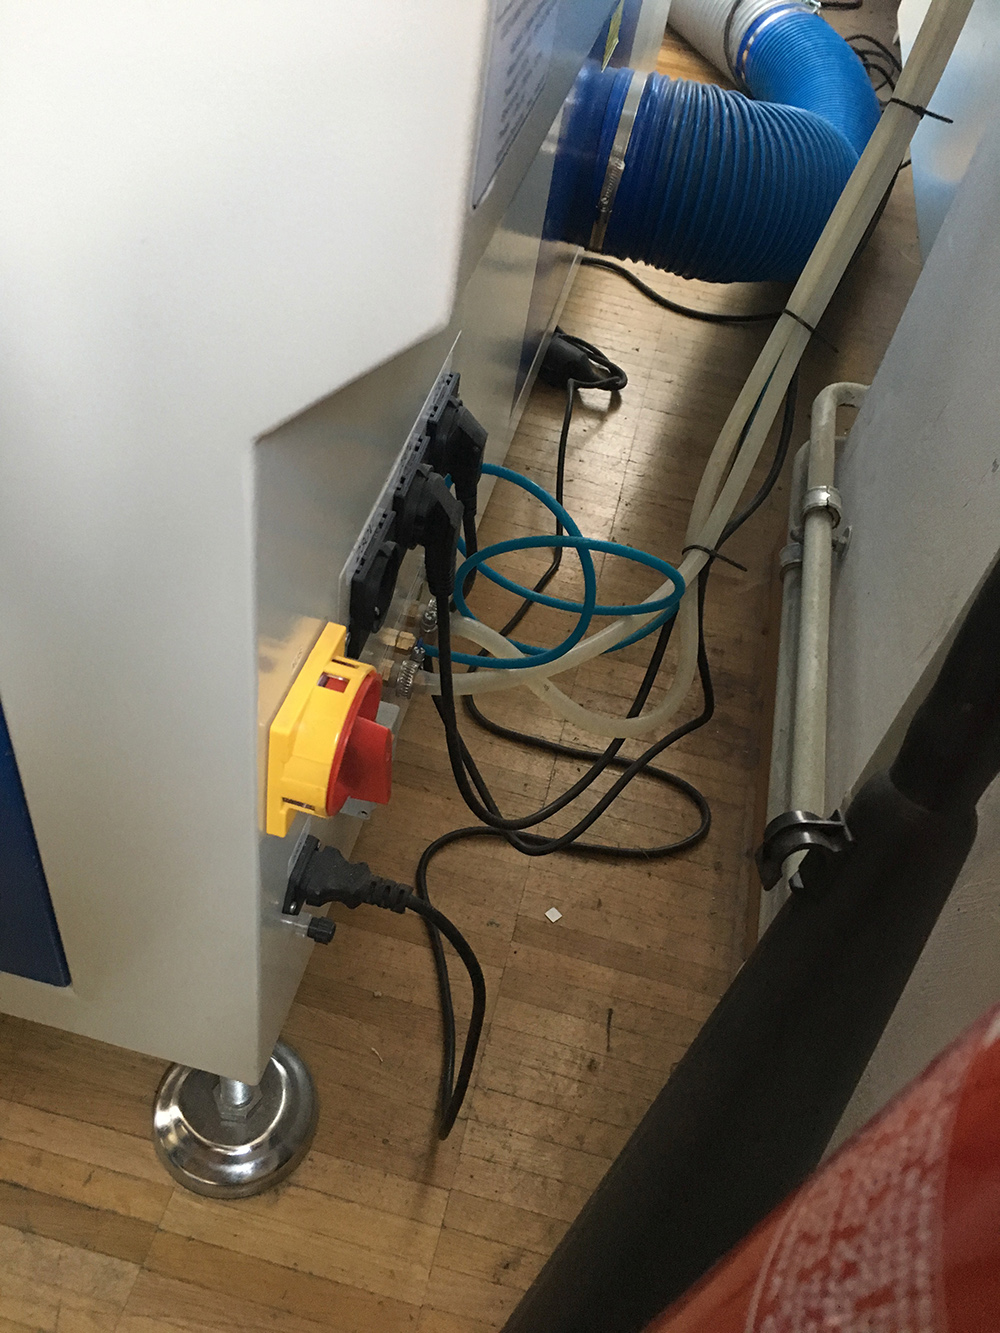
\includegraphics{assets/images/hauptschalter.jpg}
\caption{Hauptstrom}\label{fig:hauptschalter}
}
\end{figure}

Auf der Rückseite des Lasers ist ein großer rot gelber Hauptschalter
(siehe +@fig:hauptschalter). Dieser muss aktiviert werden, um der
Maschine Strom zu geben.

\hypertarget{distanztaster-uxfcberpruxfcfung}{%
\subsubsection{Distanztaster
Überprüfung}\label{distanztaster-uxfcberpruxfcfung}}

\begin{figure}
\hypertarget{fig:laserkopf}{%
\centering
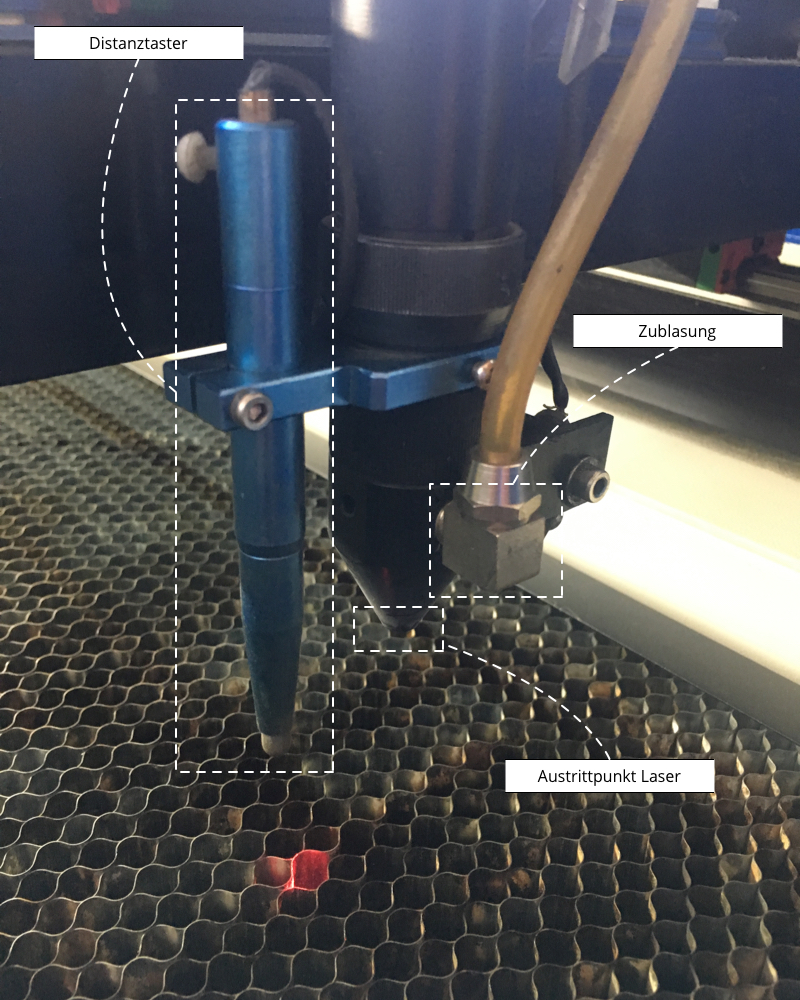
\includegraphics{assets/images/laserkopf-01.jpg}
\caption{Laserkopf mit Distanztaster}\label{fig:laserkopf}
}
\end{figure}

Am Laserkopf ist links der Distanztaster (siehe
+@fig:laserkopf).\footnote{Der Taster ähnelt einem Kugelschreiber.}
Dieser dient dazu die Distanz des Lasers zur Oberfläche des Materials
einzustellen.\footnote{Die Distanz beträgt 21,2mm.} Vor dem Einschalten
der Lasersteuerung muss überprüft werden:

\begin{enumerate}
\def\labelenumi{\arabic{enumi}.}
\tightlist
\item
  Ob der Taster sich bewegt.\footnote{Es kann passieren, dass der Taster
    verrußt und dadurch nicht mehr reagiert.}
\item
  Ob der Taster über dem Gitter beziehungsweise den Lamellen steht und
  nirgendwo anstoßen kann bei einer Referenzfahrt.
\end{enumerate}

\hypertarget{einschalten}{%
\subsubsection{Einschalten}\label{einschalten}}

\begin{figure}
\hypertarget{fig:steuerung}{%
\centering
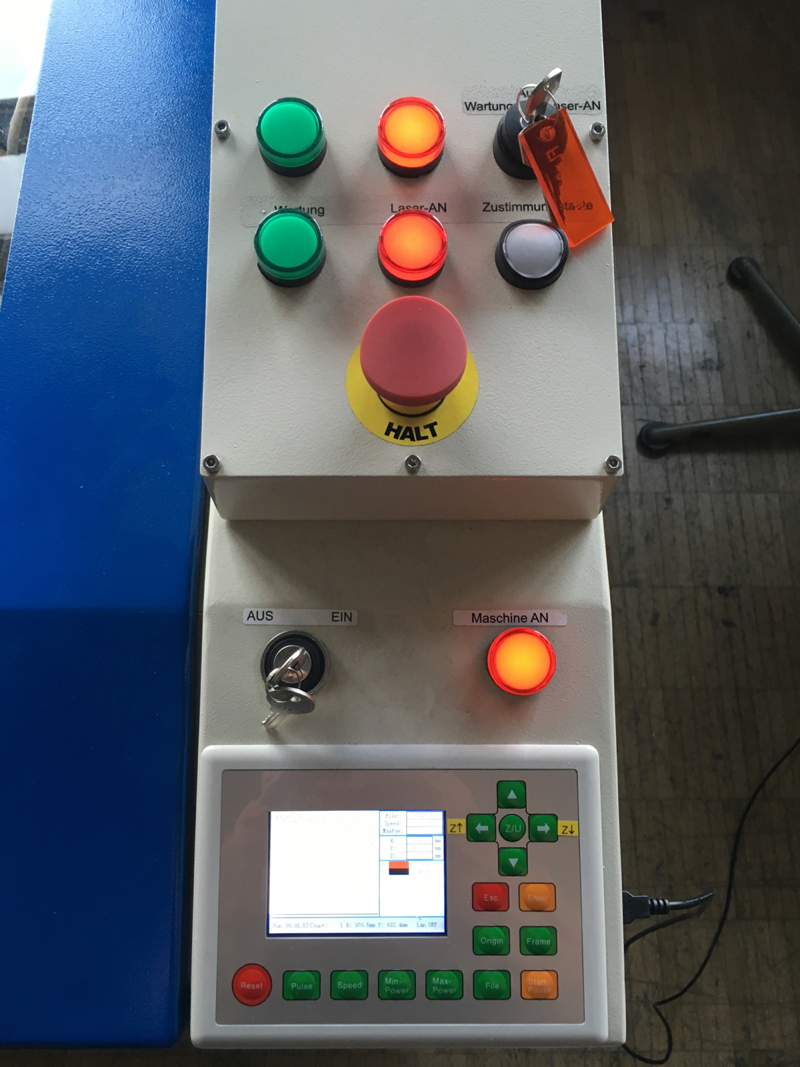
\includegraphics{assets/images/laser-control-panel.png}
\caption{Steuerung des Lasers}\label{fig:steuerung}
}
\end{figure}

Wenn alle entsprechenden Überprüfungen stattgefunden haben, kann die
Maschine über den \texttt{Aus/Ein} Drehschalter mit dem Schlüssel
aktiviert werden (siehe +@fig:steuerung unten). \textbf{Hierbei ist die
eine Hand über dem Notaus}, für den Fall, dass etwas unvorhergesehenes
passiert.\footnote{Die Referenzfahrt stoppt nicht, es wurde vergessen
  Material aus der Arbeitsfläche zu nehmen o.ä.}

\hypertarget{referenzfahrt}{%
\paragraph{Referenzfahrt}\label{referenzfahrt}}

Bei jedem Einschalten (oder nach einem
\protect\hyperlink{notaus}{Notaus}) führt die Maschine eine
Referenzfahrt in die rechte obere Ecke aus. Dies lässt sich nicht
unterbinden. Aus diesem Grund ist es besonders wichtig, beim Einschalten
die Maschine im Falle eines Problems schnell wieder abschalten zu
können. Um Probleme zu vermeiden, ist es "Best Practice" den Laserkopf
vor dem Abschalten in die rechte obere Ecke zu fahren und dort den
"\texttt{Origin}" zu setzten. Dadurch können Probleme beim nächsten
Anschalten des Anlage vermieden werden. Ebenfalls empfiehlt es sich, die
Z-Achse ein Stück abzusenken. Siehe Abschnitt "Gitter Überprüfen".

\hypertarget{z-achse}{%
\subsubsection{Z-Achse}\label{z-achse}}

\begin{figure}
\hypertarget{fig:menu}{%
\centering
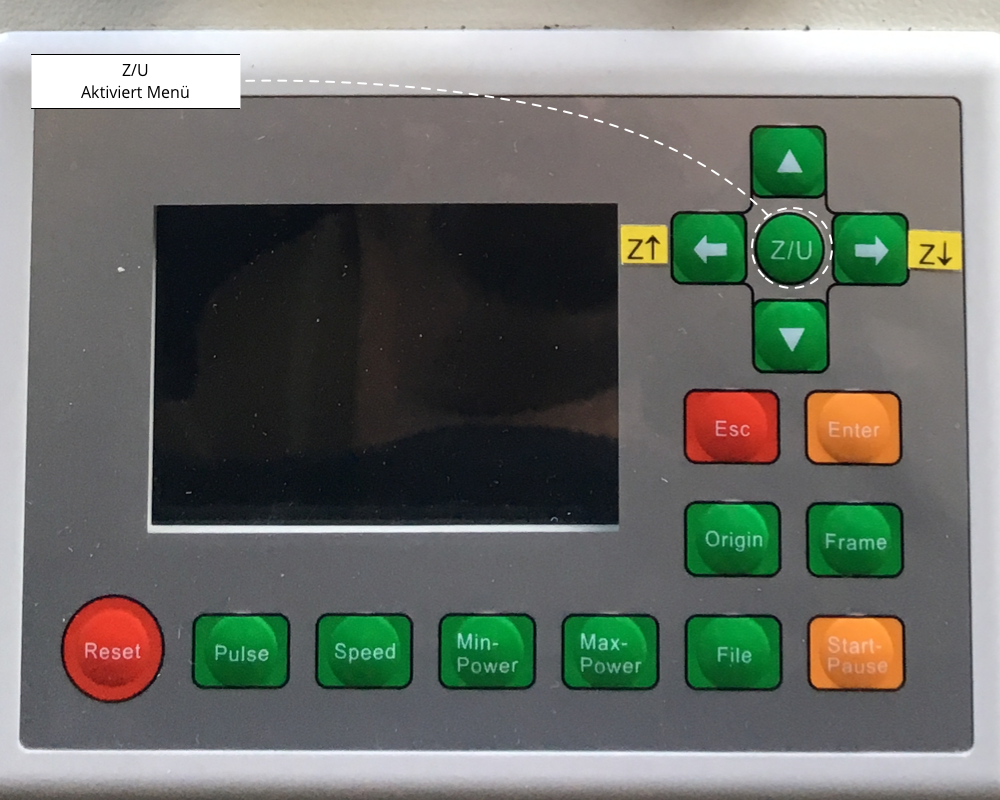
\includegraphics{assets/images/laser-menue.png}
\caption{Das Menü aktivieren}\label{fig:menu}
}
\end{figure}

\begin{figure}
\hypertarget{fig:zachse}{%
\centering
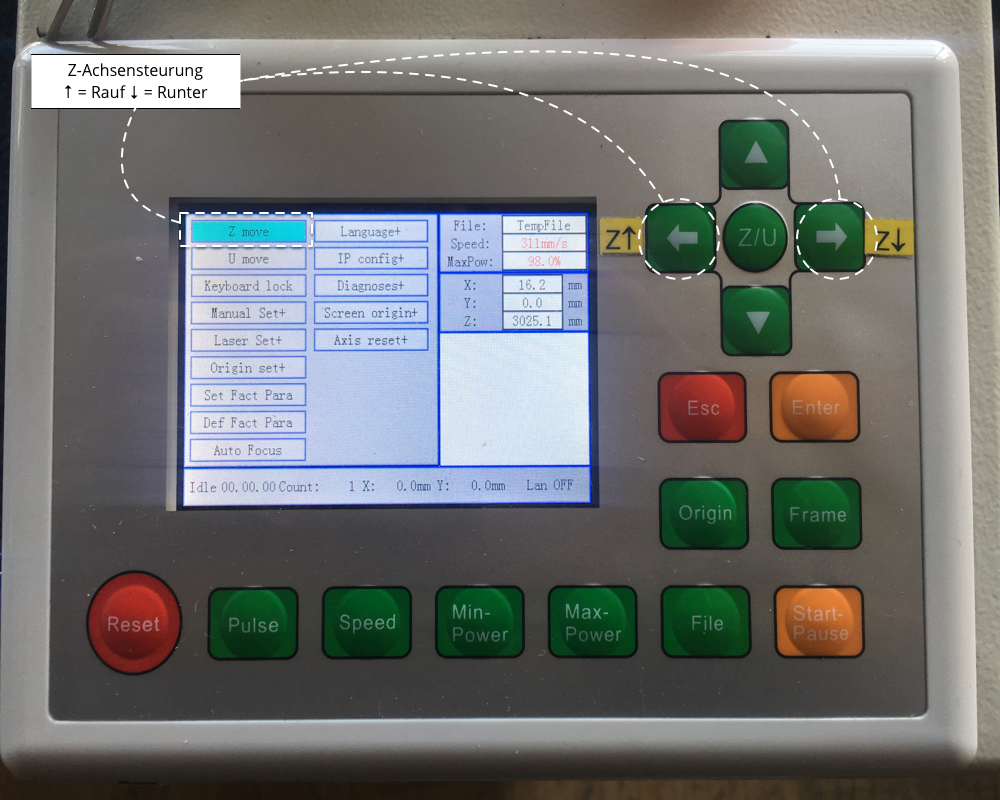
\includegraphics{assets/images/laser-z-achse.png}
\caption{Die Steuerung der Z-Achse}\label{fig:zachse}
}
\end{figure}

Die Z-Achse des Tisches kann manuell herauf oder hinunter gefahren
werden. Wenn zum Beispiel ein dickes Material eingelegt werden soll.
Dazu muss an der Steuerung (siehe +@fig:zachse) das Menü mit dem
\texttt{Z/U} (siehe +@fig:menu) Knopf in der Mitte des Steuerkreuzes
aktiviert werden. Dann können die \texttt{←} und \texttt{→} Tasten
genutzt werden um mit \texttt{←} die Z-Achse rauf zu fahren und mit
\texttt{→} runter zu fahren. Ebenfalls kann das Gitterrost
herausgenommen werden, um noch mehr Tiefe zu erzeugen.

\hypertarget{material-einlegen}{%
\subsubsection{Material Einlegen}\label{material-einlegen}}

Wenn die Maschine betriebsbereit ist, kann das zu schneidende Material
eingelegt werden. Die Arbeitsfläche der Anlage hat 1200 Millimeter (mm)
Breite und 900mm Höhe. Abhängig von der Tiefe/Stärke des Materials ist
jedoch die Fläche nicht komplett nutzbar.

Ein Beispiel: Beim Lasern einer diagonale über eine 5 × 1000 × 700mm (t
× b × h) mitteldichten Faserplatte (MDF Platte) mit einer
Geschwindigkeit von 5mm/s und einer Leistung von 95\% ist der
Laserstrahl bei ungefähr der Hälfte des Materials nicht mehr
durchgegangen.

Das bedeutet: Je stärker das Material desto kleiner wird der Bereich in
dem ein Schnitt gewährleistet ist. Es empfiehlt sich bei starken
Materialien kleinere Nutzen anzulegen und mehrere Jobs auszuführen.

\hypertarget{fokus-setzen}{%
\subsubsection{Fokus Setzen}\label{fokus-setzen}}

\begin{figure}
\hypertarget{fig:autofokus}{%
\centering
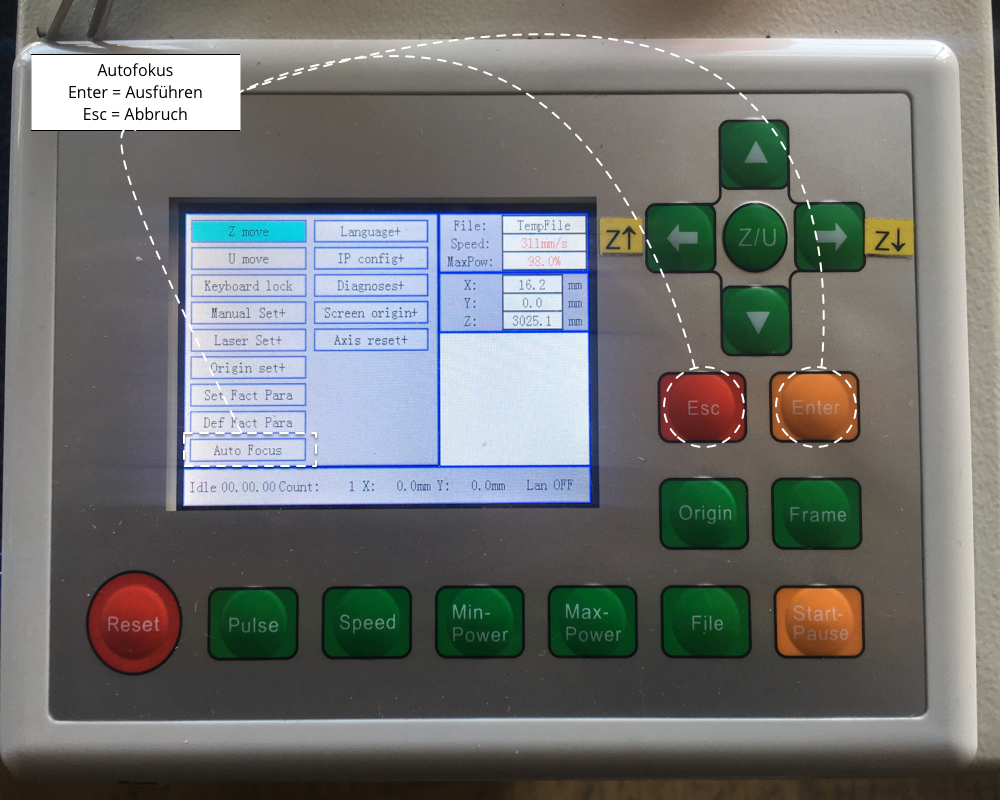
\includegraphics{assets/images/laser-autofokus.png}
\caption{Der Menüeintrag für den Autofokus}\label{fig:autofokus}
}
\end{figure}

Um den Laserkopf in seiner Distanz zur Oberfläche des Materials
einzustellen, hat die Maschine eine Autofokus Funktion. Dazu wird der
Distanztaster\footnote{Der Taster ähnelt einem Kugelschreiber.} (siehe
+@fig:laserkopf) mit dem Steuerkreuz in die Mitte des Materials
gefahren.

\textbf{Achtung:} Es empfiehlt sich bei geöffneter Klappe zu
fokussieren. Ein üblicher Fehler, den es jedoch zu vermeiden gilt, ist
dass nicht der Taster über das Material gesetzt wird sondern der
Laserpunkt. Das könnte zur Folge haben, dass der Distanztaster im Gitter
versenkt wird.\footnote{Wenn der Distanztaster im Gitter steckt bleibt
  die Maschine Abgeschaltet und muss erst wird erst wieder durch die
  zuständigen Personen freigegeben werden.} Gegebenenfalls muss die
Z-Achse noch runter gefahren werden, wenn dies nicht schon beim Einlegen
des Materials passiert ist (siehe Abschnitt
\protect\hyperlink{z-achse}{Z-Achse}). Ebenfalls sollte drauf geachtet
werden, dass das Werkstück nicht kippen kann.\\
Wenn das Material unter dem Taster liegt, kann das Menü über die Z/U
Taste aktiviert werden (siehe +@fig:menu). Mit dem Punkt
\texttt{Autofocus} (siehe +@fig:autofokus) wird die Distanz automatisch
auf 21,2mm eingestellt. Über die \texttt{↑\ ↓} Tasten kann der Punkt
Autofocus ausgewählt werden. Mit \texttt{Enter} wird er aktiviert.

\textbf{Achtung:} Beim Einstellen des Autofokus sollte immer ein Finger
auf dem \texttt{Esc} (Escape) Knopf liegen, für den Fall, dass etwas
unvorhergesehenes passiert (Der Taster bohrt sich durch das Material,
der Taster reagiert nicht, der Taster ist doch nicht über dem Material).

Nach dem Autofokus Prozess liegt der Brennpunkt des Lasers auf der
Oberfläche des Materials.\footnote{Bei starken Materialien kann es
  nützlich sein den Fokus nicht auf der Oberfläche, sondern im Material
  zu haben. Um bei einem 10mm starken Material dies zu bewerkstelligen,
  bedarf es eines 5mm starken Materials. Auf dieses wird der Fokus
  gesetzt. Dann wird es durch das 10mm starke Material ausgetauscht.
  Hierbei ist jedoch drauf zu achten, dass der Taster nicht gegen das
  Material stoßen darf. Diese Methode ist nur ratsam für bereits
  erfahrene Benutzer.}

\hypertarget{null-null-origin}{%
\subsubsection{\texorpdfstring{Null Null
(\texttt{Origin})}{Null Null (Origin)}}\label{null-null-origin}}

\begin{figure}
\hypertarget{fig:origin}{%
\centering
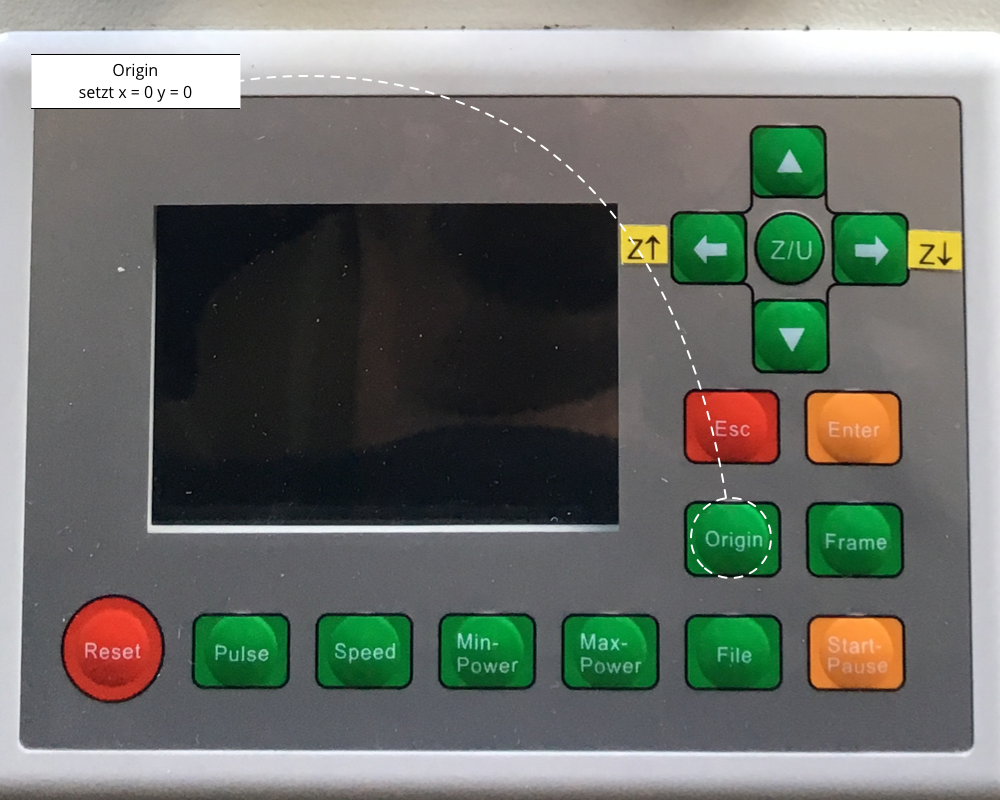
\includegraphics{assets/images/laser-origin.png}
\caption{Setzten des Origins}\label{fig:origin}
}
\end{figure}

Um die Maschine für den Laser Job bereits zu haben, kann nun der
Laserkopf mit den \texttt{←\ ↑\ ↓\ →} Tasten an die gewünschte Position
gefahren werden. Um diese Position als Ausgangspunkt für einen Schnitt,
eine Gravur oder eine Perforation zu setzten, muss dies mit der Taste
"\texttt{Origin}" (siehe +@fig:origin) bestätigt werden.\footnote{Die
  Taste bestätigt, dass sie gedrückt wurde mit einem Piep. Mehr nicht.
  Es empfiehlt sich vor einem Job mehrfach zu überprüfen, ob der
  \texttt{Origin} auch gesetzt ist.} Falls Unsicherheit besteht ob der
\texttt{Origin} auch der aktuellen Position des Laserkopfes entspricht,
kann über einen Druck auf die Taste \texttt{Esc} der Kopf auf seinen
letzten \texttt{Origin} zurückgesetzt werden.

\textbf{Achtung:} Vor dem Starten eines Jobs sollte nochmals
sichergestellt werden, dass der \texttt{Origin} stimmt. Der Laser
beginnt einen Job von dieser Position aus (siehe Abschnitt
\protect\hyperlink{positionierung}{Positionierung}). Falls die Position
vom \texttt{Origin} abweicht, könnte das Material an einer anderen
Stelle bearbeitet werden.

\hypertarget{laser-job}{%
\subsection{Laser Job}\label{laser-job}}

Die einfachste Methode einen Job zu starten ist, über die USB Verbindung
aus der RDWorks Software heraus mit der Start Taste. Es existiert auch
die Möglichkeit Job Dateien aus RDWorks heraus auf ein USB Stick zu
speichern und diesen direkt in die Maschine zu stecken. Dafür muss der
Stick FAT formatiert sein und die Dateien müssen auf der untersten Ebene
des Dateisystems liegen. Unterordner werden nicht erkannt. Im weiteren
Verlauf dieses Handbuches wird diese Möglichkeit nicht berücksichtigt.
Ebenfalls werden hier nur die minimalen Schritte beschrieben um einen
Job mit RDWorks einzurichten und auszuführen. Ein komplette Übersicht
würde den Rahmen diese Dokuments sprengen. Hierfür existiert ein
Benutzerhandbuch, das vom Hersteller der Software zusammen mit dieser
ausgeliefert wird.

\hypertarget{positionierung}{%
\subsubsection{Positionierung}\label{positionierung}}

Der \protect\hyperlink{null-null-origin}{Origin} des Laserkopfes
korrespondiert mit der linken oberen Ecke der Daten in der Software
(siehe +@fig:rdsoftware). Dies sollte nicht verändert werden, da die
Leistung des Lasers von Links oben nach rechts unten abnimmt.\footnote{Versuche
  mit einer 3mm starken 700mm × 1000mm MDF Platte haben gezeigt, dass
  bei einer Leistung von 95\% und einer Geschwindigkeit von 5mm/s die
  Platte mit einem diagonalen Schnitt nur bis zur Hälft geschnitten
  werden kann.} Wenn die Daten die mögliche zu fahrende Fläche
überschreitet, wird dies im Menü angezeigt. Es ist möglich den Job
dennoch durchführen zu lassen. Alles was über die Arbeitsfläche hinaus
geht wird nicht gelasert.

\hypertarget{die-parameter-verstehen}{%
\subsubsection{Die Parameter Verstehen}\label{die-parameter-verstehen}}

Die Parameter die zur Verfügung stehen sind

\begin{enumerate}
\def\labelenumi{\arabic{enumi}.}
\tightlist
\item
  Die Geschwindigkeit des Laserkopfes gemessen in Millimeter pro Sekunde
  (mm/s).
\item
  Die Intensität des Laserstahls gemessen in Prozent (\%).
\end{enumerate}

Ausgehend von diesen beiden Parametern muss der Job eingerichtet werden.
Ein 3mm Acrylplatte würde zum Beispiel bei 10mm/s und 90\% Leistung
geschnitten werden. Eine Gravur auf dieser Platte kann schon bei 80mm/s
und 15\% Leistung gut aussehen.

Stärkere Materialien bedürfen mehr Leistung und eine langsamere
Bewegung. Dünne Materialien können bei einer schnellen Fahrt auch schon
mit geringer Leistung geschnitten werden. Wobei eine zu hohe
Geschwindigkeit sich auch auf die Qualität von Kurven und Ecken
auswirkt. Es gilt hier eigenen Erfahrungswerte zu sammeln. Ebenfalls
können die Außentemperatur, die Feuchtigkeit des Materials oder auch die
Reinigung der Umwerf-Spiegel die Werte beeinflussen.

\hypertarget{daten-vorbereiten}{%
\subsubsection{Daten Vorbereiten}\label{daten-vorbereiten}}

Die Steuerungssoftware RDWorks kann mit zwei unterschiedlichen
Dateitypen umgehen.

\begin{enumerate}
\def\labelenumi{\arabic{enumi}.}
\tightlist
\item
  Vektor Daten
\item
  Pixel Bilder
\end{enumerate}

\hypertarget{vektor-daten}{%
\subsubsection{Vektor Daten}\label{vektor-daten}}

Vektor Daten können für das Schneiden, Perforieren und Gravieren genutzt
werden. Es existieren einige Applikationen zum Erstellen von
Vektordaten. Adobe Illustrator (AI),
\href{https://inkscape.org/en/}{Inkscape}, Affinity Designer, Sketch.
Hier werden Beispiele aus AI gezeigt.

Für Schnitt und Perforation können Pfade angelegt werden, die offen
sind. Diese werden von dem Laserkopf nachgefahren. Hierbei ist zu
beachten, dass die Software jeden Pfad erkennt, der im Dokument liegt.
Es werden nur Pfade erkannt, keine Konturen. In +@fig:ai-kontur ist die
GPU-Vorschau von AI zu sehen. Dies ist jedoch nicht, was der Laser
erkennt.

\begin{figure}
\hypertarget{fig:ai-kontur}{%
\centering
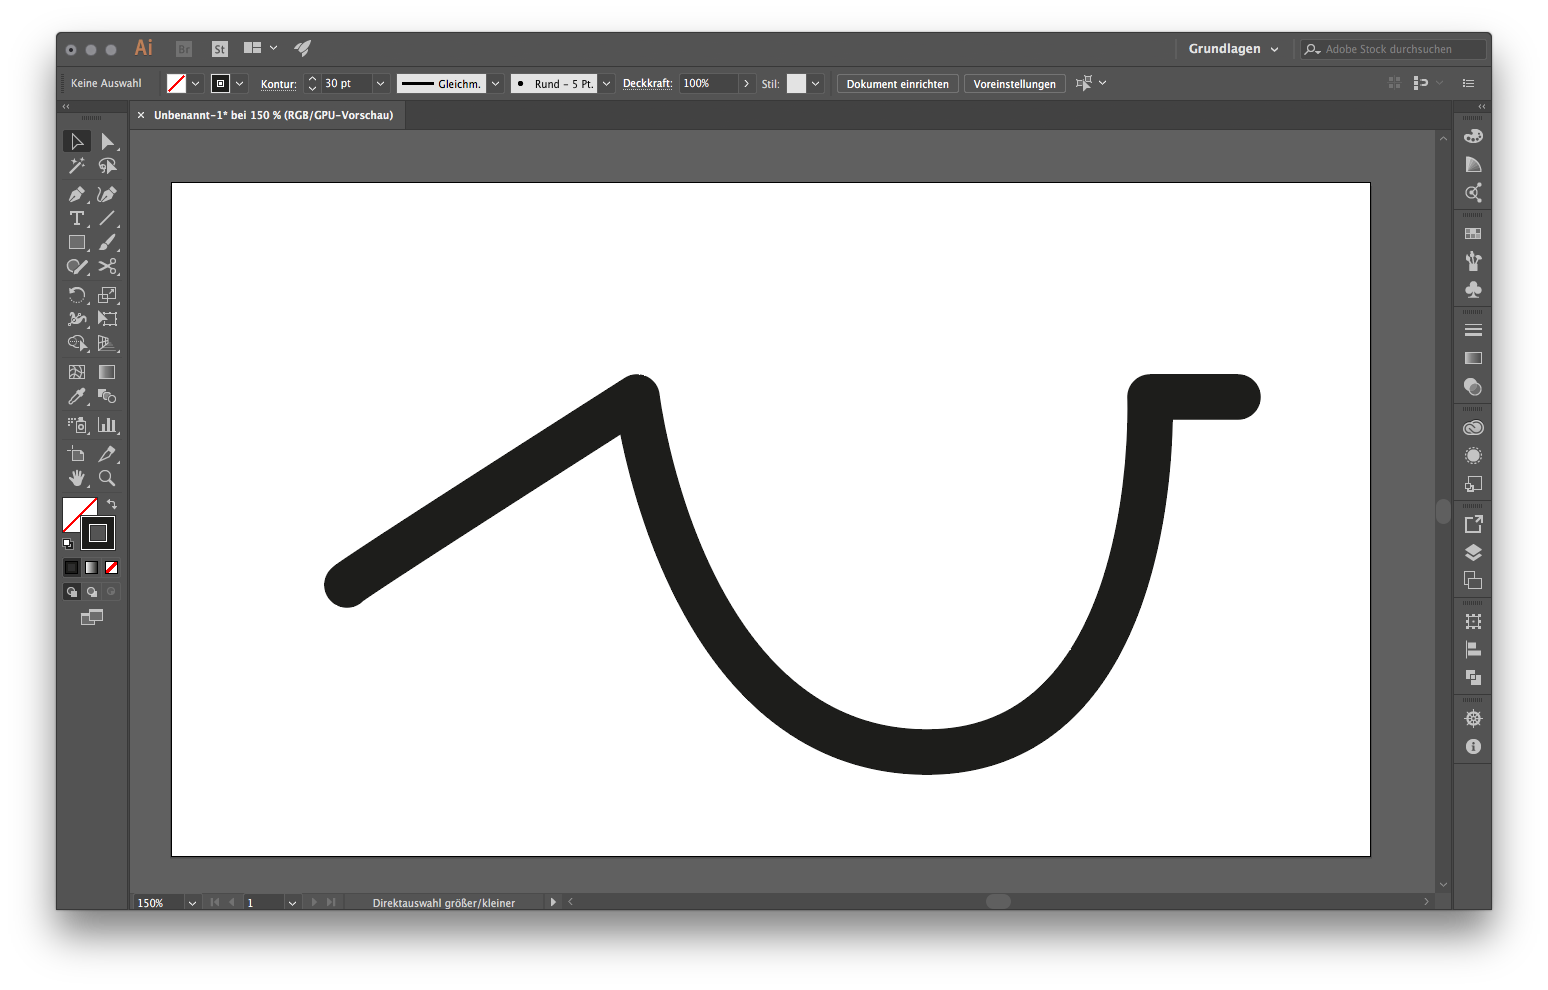
\includegraphics{assets/images/ai-kontur.png}
\caption{Adobe Illustrator GPU-Vorschau}\label{fig:ai-kontur}
}
\end{figure}

Was in +@fig:ai-pfad zu sehen ist, entspricht dem, was von dem Laserkopf
nach fahren würde. Die Abbildung zeigt die Pfadansicht. Um zwischen
GPU-Vorschau und Pfadansicht zu wechseln kann die Tastenkombination
\texttt{Command\ Y} (macOS) oder \texttt{Strg\ Y} (Win) genutzt
werden.\footnote{Im weiteren Verlauf dieses Handbuchs wird nur die macOS
  Variante \texttt{Command} dargestellt. Für Windows muss dies durch
  \texttt{Strg} ersetzt werden. Falls Abweichungen existieren wird
  darauf hingewiesen.}

\begin{figure}
\hypertarget{fig:ai-pfad}{%
\centering
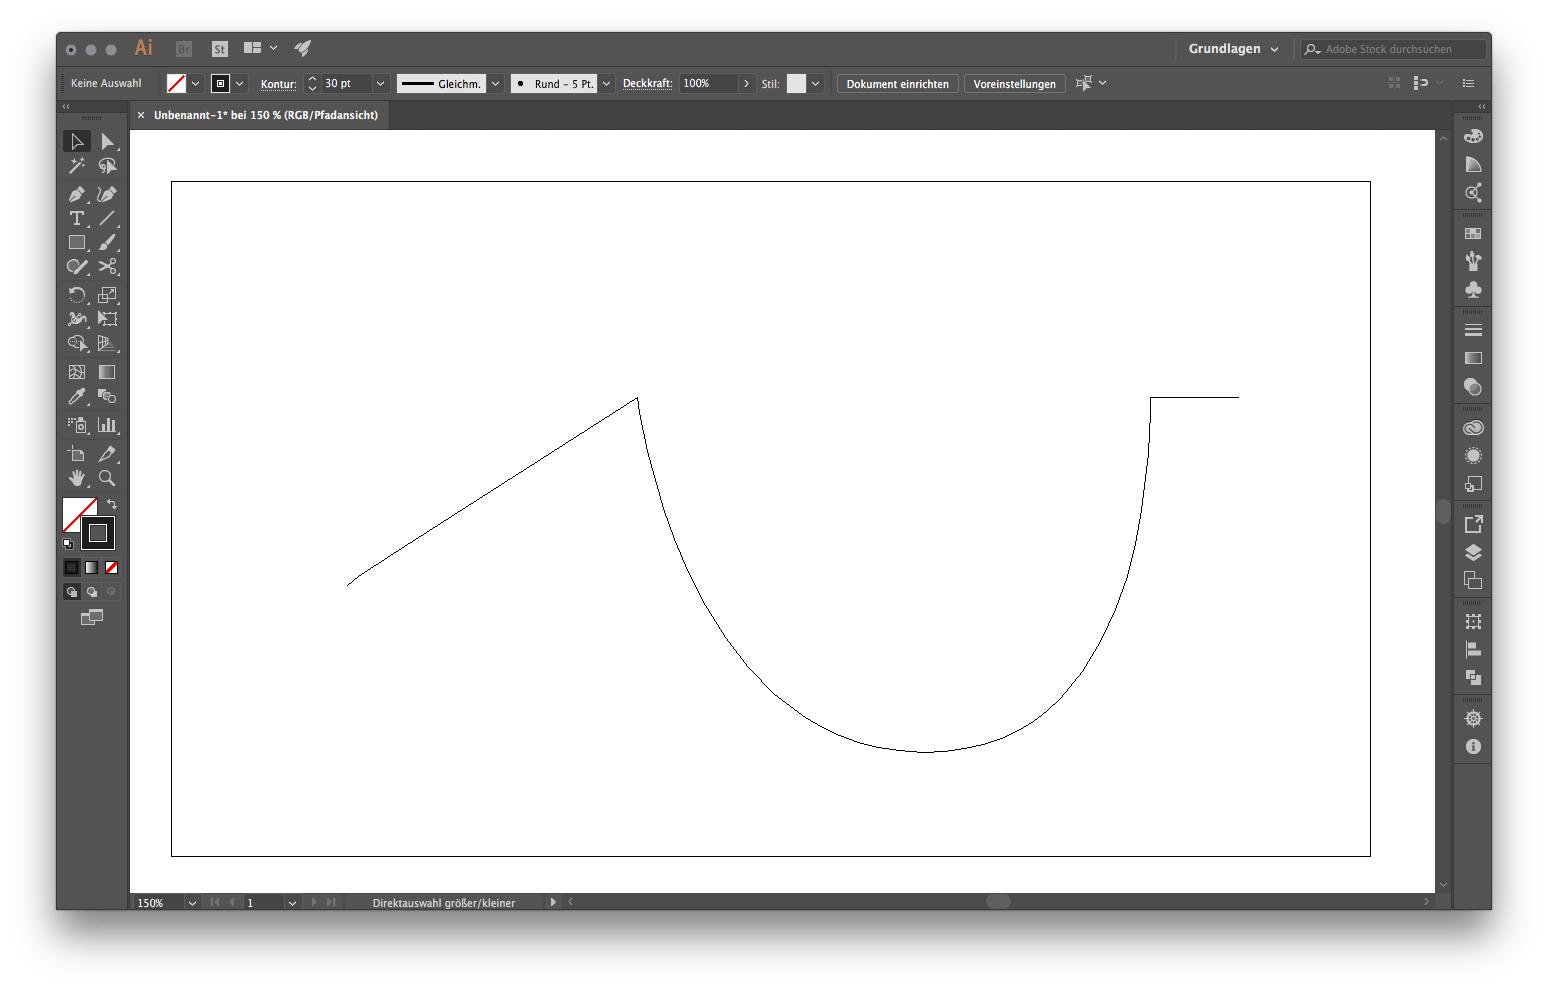
\includegraphics{assets/images/ai-pfad.png}
\caption{Adobe Illustrator Pfad Ansicht}\label{fig:ai-pfad}
}
\end{figure}

Für die Gravuren funktionieren nur geschlossene Vektorpfade. In
+@fig:offengpu sieht es so aus, als ob beide Flächen geschlossen sind.
Die Pfadansicht zeigt jedoch, dass die rechte Form nicht geschlossen ist
+@fig:offen. Somit würde die rechte Form für eine Gravur nicht beachtet
werden.

\begin{figure}
\hypertarget{fig:offengpu}{%
\centering
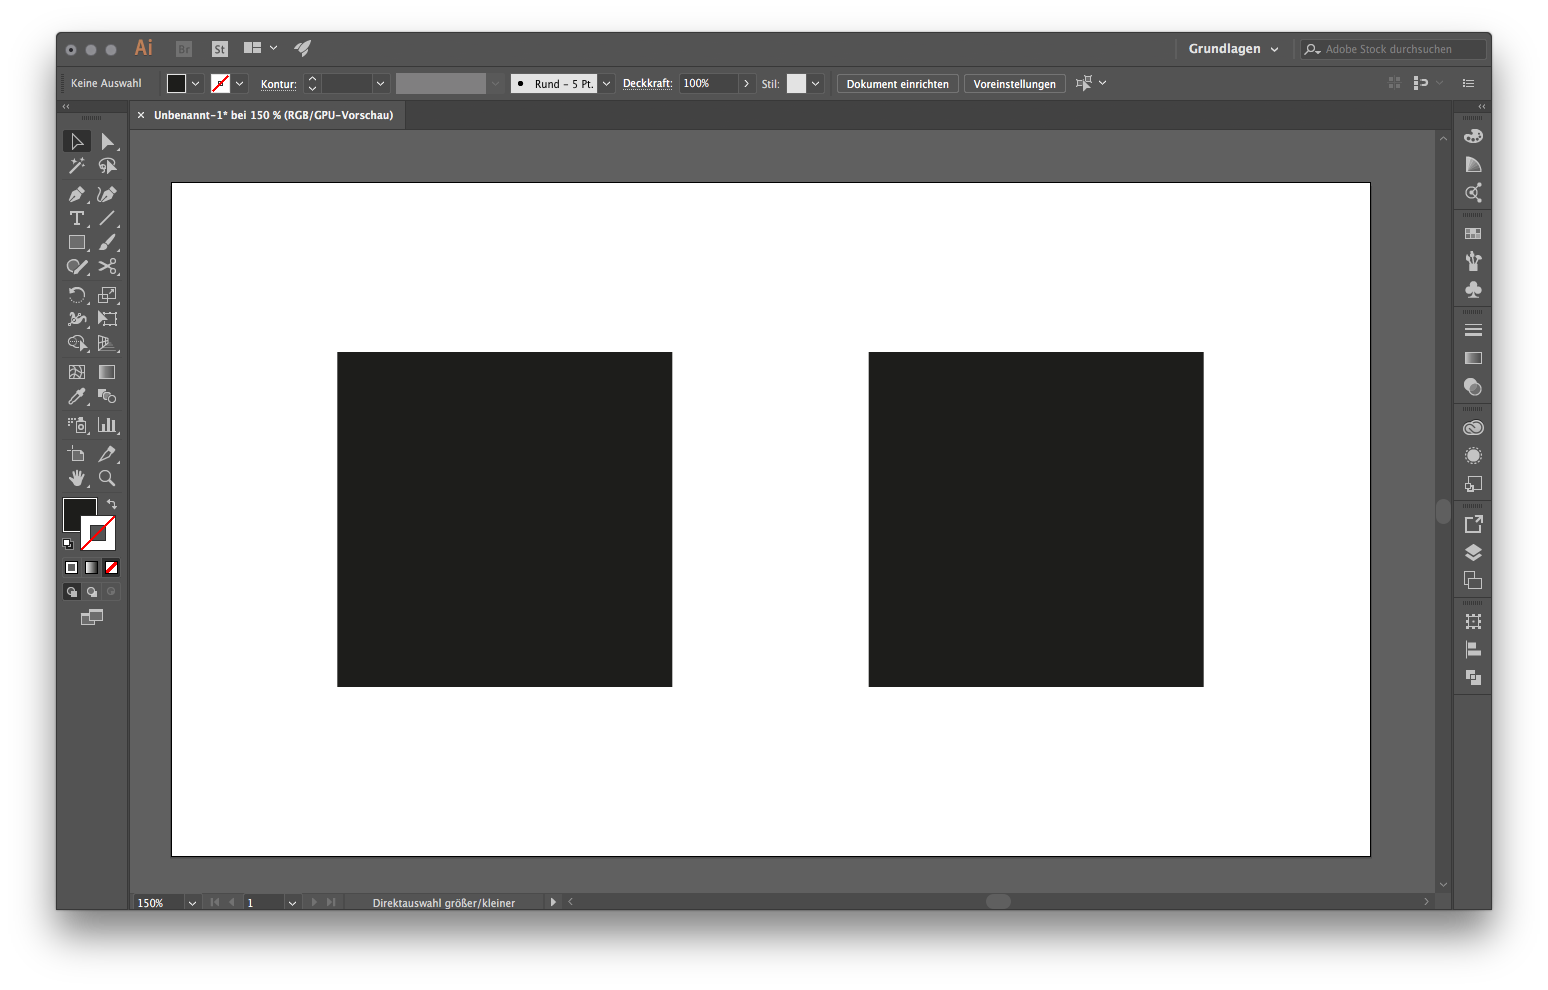
\includegraphics{assets/images/ai-flaeche-offen-gpu.png}
\caption{Adobe Illustrator Fläche offen
GPU-Vorschau}\label{fig:offengpu}
}
\end{figure}

\begin{figure}
\hypertarget{fig:offen}{%
\centering
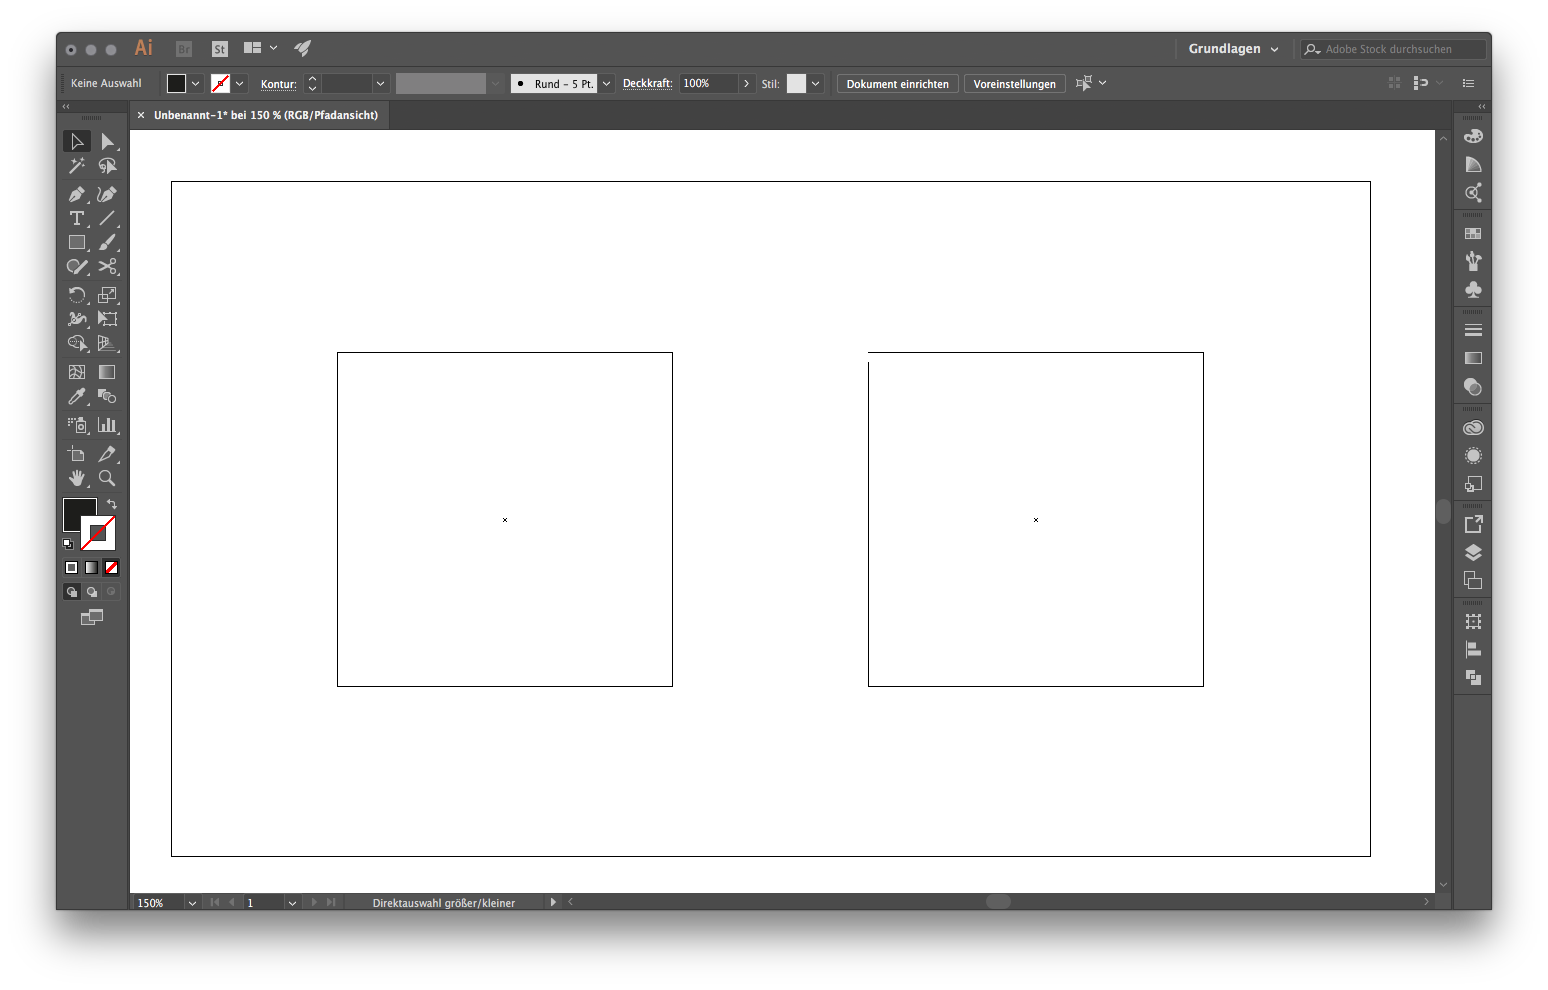
\includegraphics{assets/images/ai-flaeche-offen.png}
\caption{Adobe Illustrator Fläche offen Pfadansicht}\label{fig:offen}
}
\end{figure}

\newpage

Grundsätzlich sollte ein AI Dokument so angelegt werden, dass

\begin{itemize}
\tightlist
\item
  keine Überreste von Pfadpunkten in ihm liegen.
\item
  keine Ebenen ausgeblendet werden.
\item
  keine Daten außerhalb der Arbeitsfläche liegen.
\end{itemize}

\begin{figure}
\hypertarget{fig:reste-gpu}{%
\centering
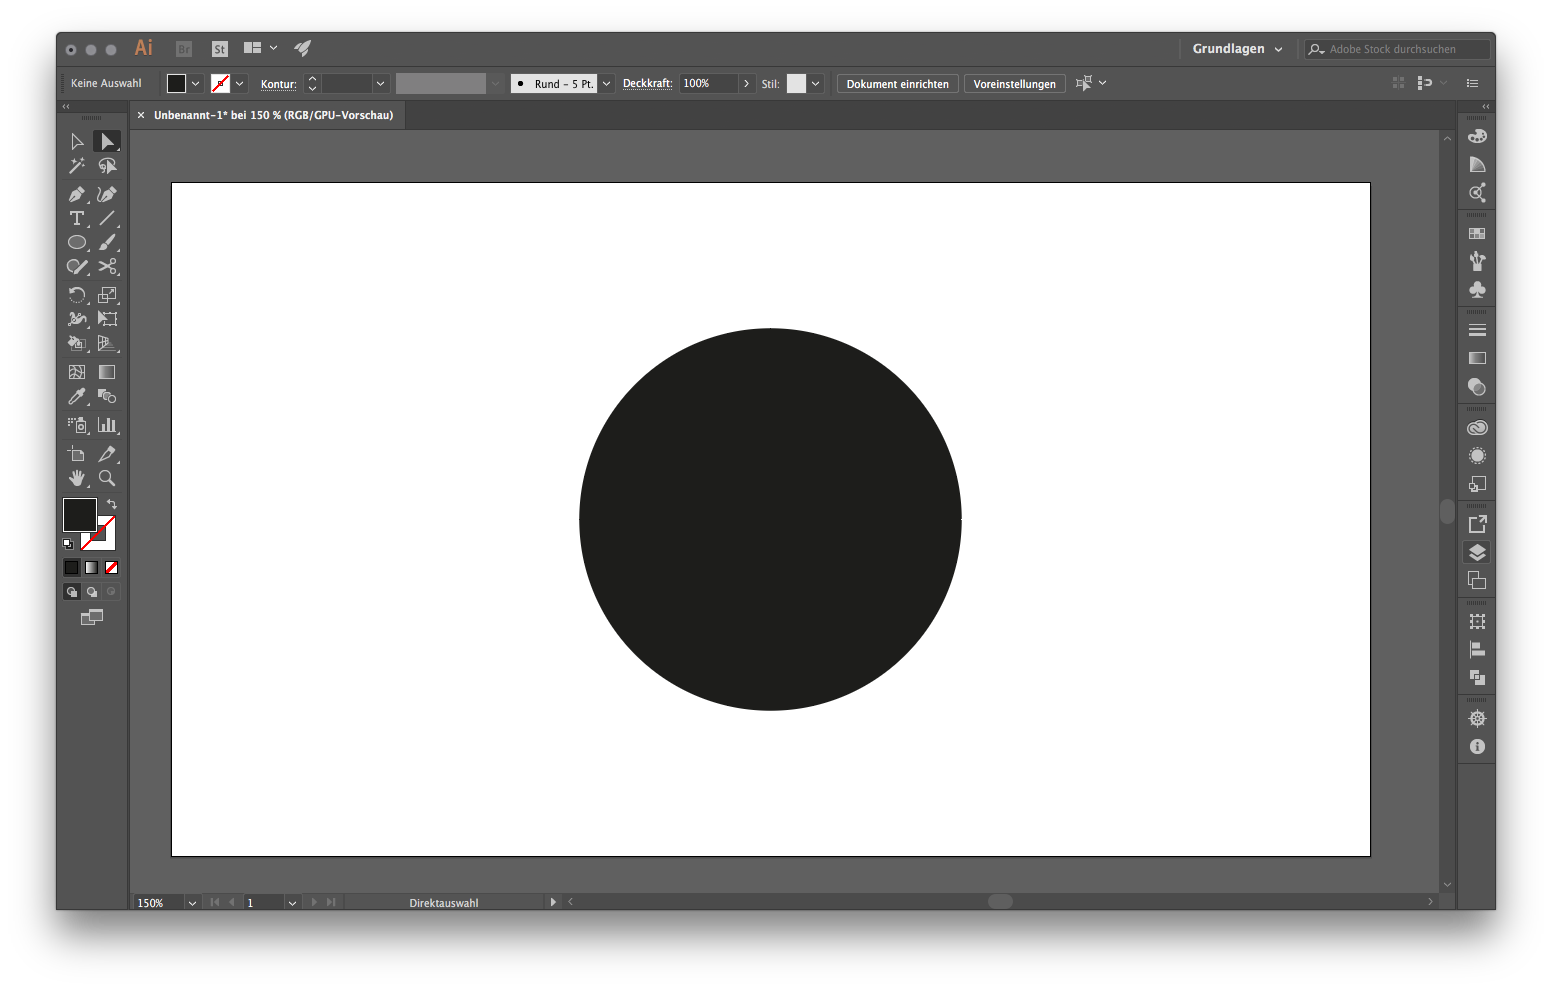
\includegraphics{assets/images/ai-reste-gpu.png}
\caption{Adobe Illustrator versteckte Reste
GPU-Vorschau}\label{fig:reste-gpu}
}
\end{figure}

\begin{figure}
\hypertarget{fig:reste}{%
\centering
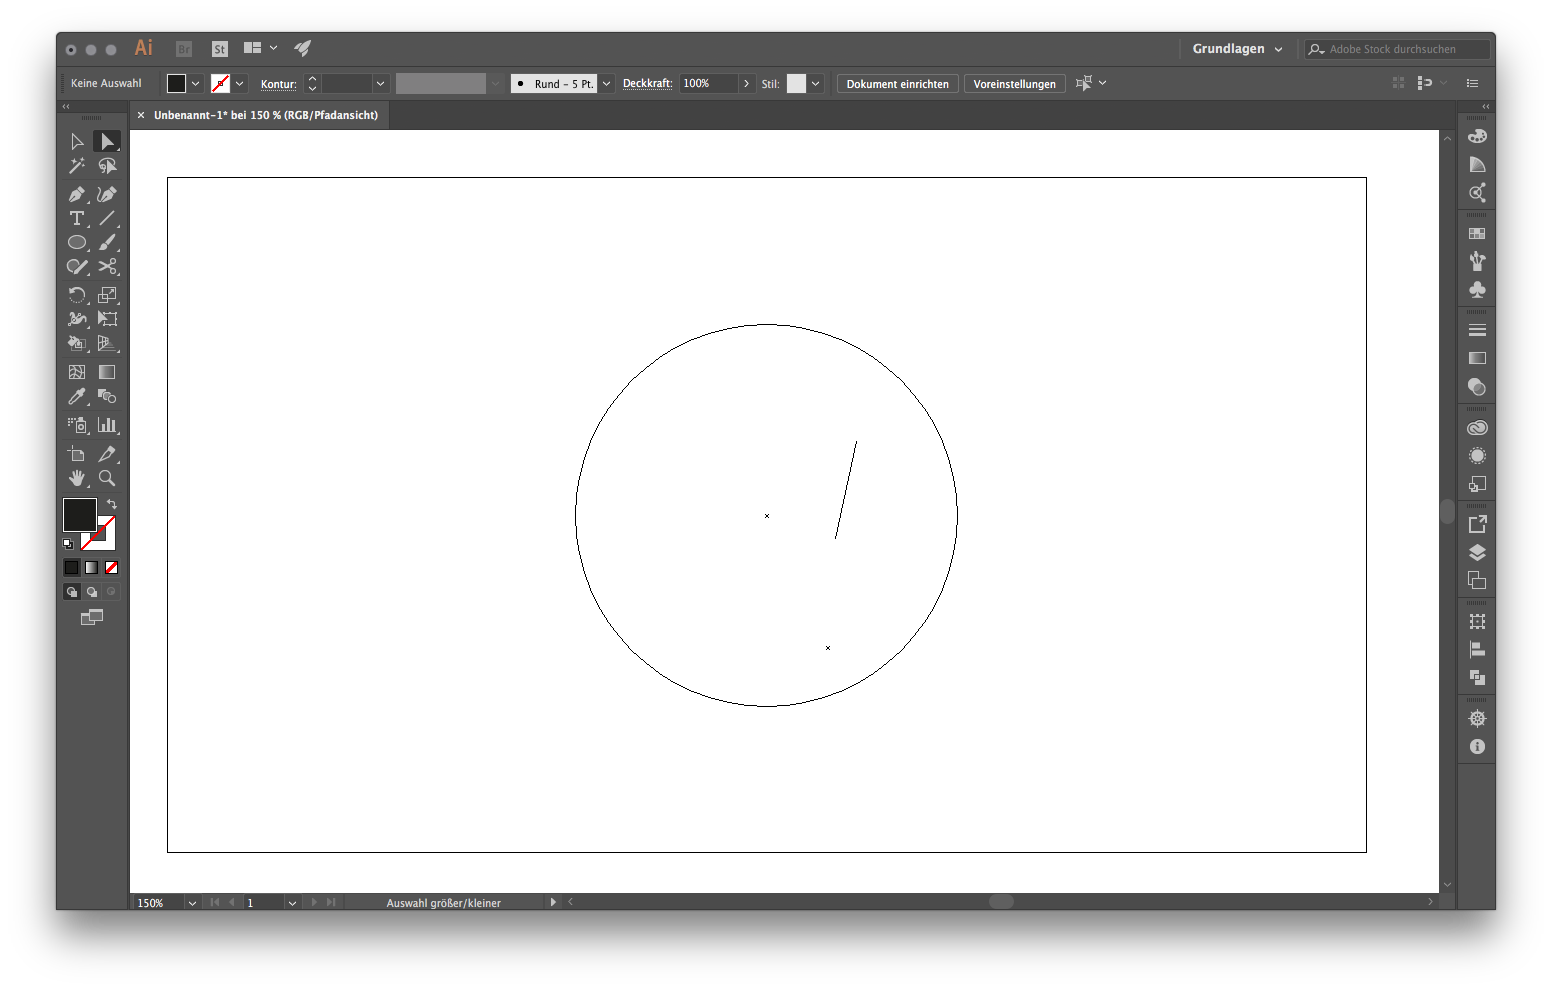
\includegraphics{assets/images/ai-reste.png}
\caption{Adobe Illustrator versteckte Reste
Pfadansicht}\label{fig:reste}
}
\end{figure}

In +@fig:reste-gpu und +@fig:reste sind in der Pfadansicht Reste zu
sehen, die optisch in der GPU-Vorschau nicht zu erkennen wären. Die
Maschine würde diese Pfadpunkte und Pfade dennoch in Betracht ziehen.

\hypertarget{unterstuxfctzte-vektor-formate}{%
\paragraph{Unterstützte Vektor
Formate}\label{unterstuxfctzte-vektor-formate}}

Die Software RDworks unterstützt viele Formate. Die besten Ergebnisse
wurden bisher mit folgenden Formaten erzielt.\footnote{Weiter
  Informationen zu Formaten sind im Handbuch der Software zu finden.}

\begin{itemize}
\tightlist
\item
  .ai (Version 3)
\item
  .dxf (R14)
\end{itemize}

Bei allen Formaten ist zu beachten, dass die voreingestellte Einheit mm
sein sollte.

\hypertarget{limitierungen-von-vektorformaten}{%
\paragraph{Limitierungen von
Vektorformaten}\label{limitierungen-von-vektorformaten}}

Wenn man die Pfade durch Code generiert
(\href{https://processing.org/}{Processing},
\href{https://p5js.org/}{p5js}, etc.), muss man auf die Länge der Pfade
(Anzahl Punkte) achten. Sowohl Programme wie Illustrator als auch
RD\_Works selber haben hier Limits. Bei beiden Programmen ist nicht
wirklich dokumentiert, was diese Limits sind. Hier muss man darauf
achten entweder die Anzahl Punkte reduzieren, oder die Pfade in mehrere
Unterpfade aufbrechen.

\hypertarget{ai-dxf-export}{%
\paragraph{AI DXF Export}\label{ai-dxf-export}}

\begin{figure}
\hypertarget{fig:ai-datei-dialog}{%
\centering
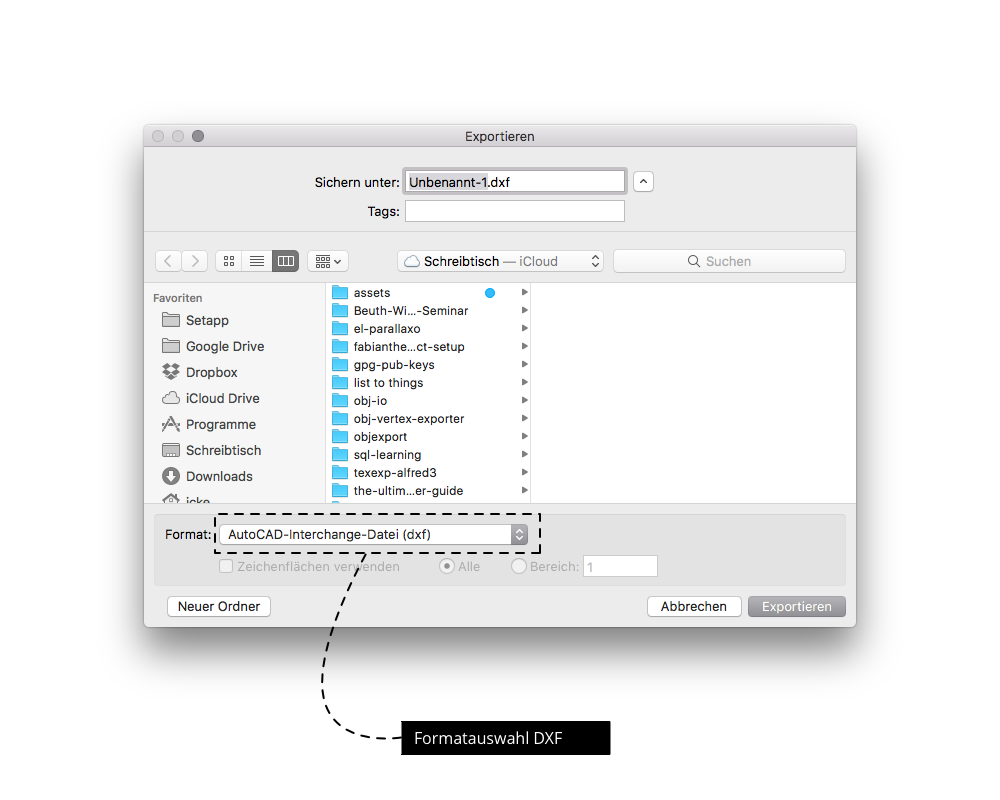
\includegraphics{assets/images/ai-datei-dialog.png}
\caption{Adobe Illustrator Datei Export
Dialog}\label{fig:ai-datei-dialog}
}
\end{figure}

DXF Dateien können aus AI unter
\texttt{Datei\textgreater{}Exportieren\textgreater{}Exportieren\ als\ldots{}}
ausgegeben werden. Dazu muss am unteren Rand des Datei Dialogs die
Option \texttt{AutoCAD-Interchange-Format\ (DXF)} gewählt werden. Siehe
+@fig:ai-datei-dialog.\\
Dies öffnet einen weiteren Dialog für die Einstellungen der DXF Datei.
Hier ist drauf zu achten, dass

\begin{itemize}
\tightlist
\item
  die AutoCAD Version \texttt{R14/LT98/LT97} ist.
\item
  im Abschnitt \texttt{Bildmaterialskalierung} die Einheiten richtig von
  1 mm in 1 Einheit skaliert werden.
\end{itemize}

Alle weiteren Einstellungen können so bleiben, wie sie sind. (Siehe
+@fig:dxf-ex)

\begin{figure}
\hypertarget{fig:dxf-ex}{%
\centering
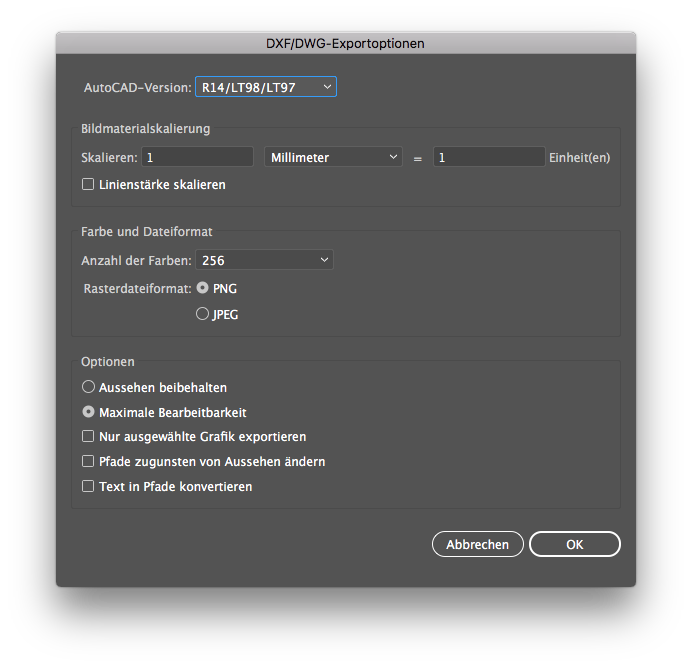
\includegraphics{./assets/images/ai-dxf-export-dialog.png}
\caption{Adobe Illustrator DXF Export Dialog}\label{fig:dxf-ex}
}
\end{figure}

\hypertarget{daten-trennen}{%
\subparagraph{Daten Trennen}\label{daten-trennen}}

Wenn in einer Datei mehrere Arten von Schnitt, Perforation oder Gravur
angelegt werden sollen, können die einzelnen Objekte getrennt werden,
indem ihnen eine eigene Farbe zugeordnet wird. Ebenen werden beim Export
nicht berücksichtigt.

\hypertarget{pixelbilder}{%
\subsubsection{Pixelbilder}\label{pixelbilder}}

Es können ebenfalls Pixelbilder genutzt werden, um Gravuren zu erzeugen.
Hierbei besteht die Möglichkeit die Graustufen des Bildes zu verwenden,
um die Intensität des Lasers zu steuern. Die Bilder können maximal einen
Auflösung von 1000 "dots per inch" (dpi) haben. Ab 300dpi können bereits
sehr gute Ergebnisse erzielt werden. Unterhalb von 300dpi wird die
Auflösung der Gravur roh. Gerade bei Schriften sollte wenn möglich
entweder eine hohe Auflösung genutzt werden oder auf Vektoren
zurückgegriffen werden.

\hypertarget{limitierungen-bei-pixelbildern}{%
\paragraph{Limitierungen bei
Pixelbildern}\label{limitierungen-bei-pixelbildern}}

Auch wenn eine Auflösung von 1000 dpi möglich ist, gibt es ein Limit bei
der Größe der Bilder, welche bei ca. 7500x7500 Pixeln liegt.

\begin{figure}
\hypertarget{fig:moire}{%
\centering
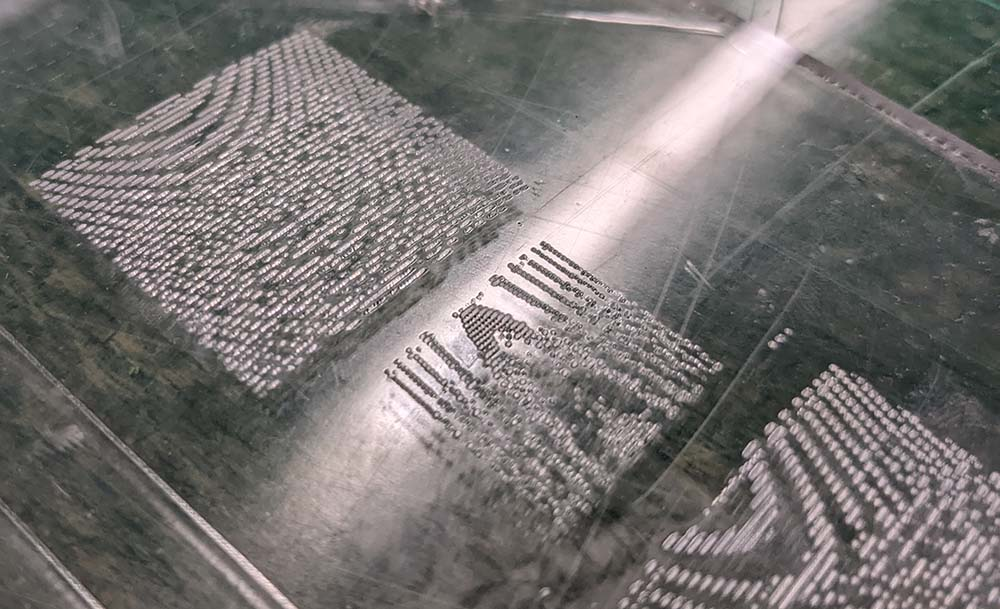
\includegraphics{./assets/images/moire.jpg}
\caption{Moire Beispiel}\label{fig:moire}
}
\end{figure}

Wenn die Rasterbilde sehr viele Linien oder Punkte enthalten, also
abwechseln dunkle und helle Pixel, kann es zu einem
\href{https://de.wikipedia.org/wiki/Moir\%C3\%A9-Effekt}{Moiré-Effekt}
kommen (siehe +@fig:moire). Zumindest nach aktuellem Erfahrungsstand
lässt sich dies nicht umgehen. Bei feinen Details die auch über
Laserschnitt erstellt werden können, gibt es aber eine Lösung: Im Menü
über \emph{Handling \textgreater{} Bitmap Handling} das Fenster für
Bitmap-Bearbeitung aufrufen. Dort Pfade generieren (Get Outline) lassen
und diese der Quelle und dem Display (Apply to view, Apply to source)
zuweisen. Dies vektorisiert das Bitmap. Dabei ist zu beachten, das aus
Linien Flächen werden. Wenn es sehr dünne Linien sind, ist das egal,
ABER der Laser fährt dann zweimal über jede Linie, dies sollte
entsprechend bei der Stärke beachtet werden.

\hypertarget{daten-import}{%
\subsubsection{Daten Import}\label{daten-import}}

Vektor Dateien und Pixelbilder werden über den Befehl
\texttt{Datei\textgreater{}Import} in die Software eingeladen.

\hypertarget{art-des-jobs}{%
\subsubsection{Art des Jobs}\label{art-des-jobs}}

Die Art des Laserjobs bestimmt auch mit welche Möglichkeiten zur
Verfügung stehen.

\begin{itemize}
\tightlist
\item
  Schneiden
\item
  Gravieren
\item
  Perforieren
\end{itemize}

\begin{figure}
\hypertarget{fig:rdsoftware}{%
\centering
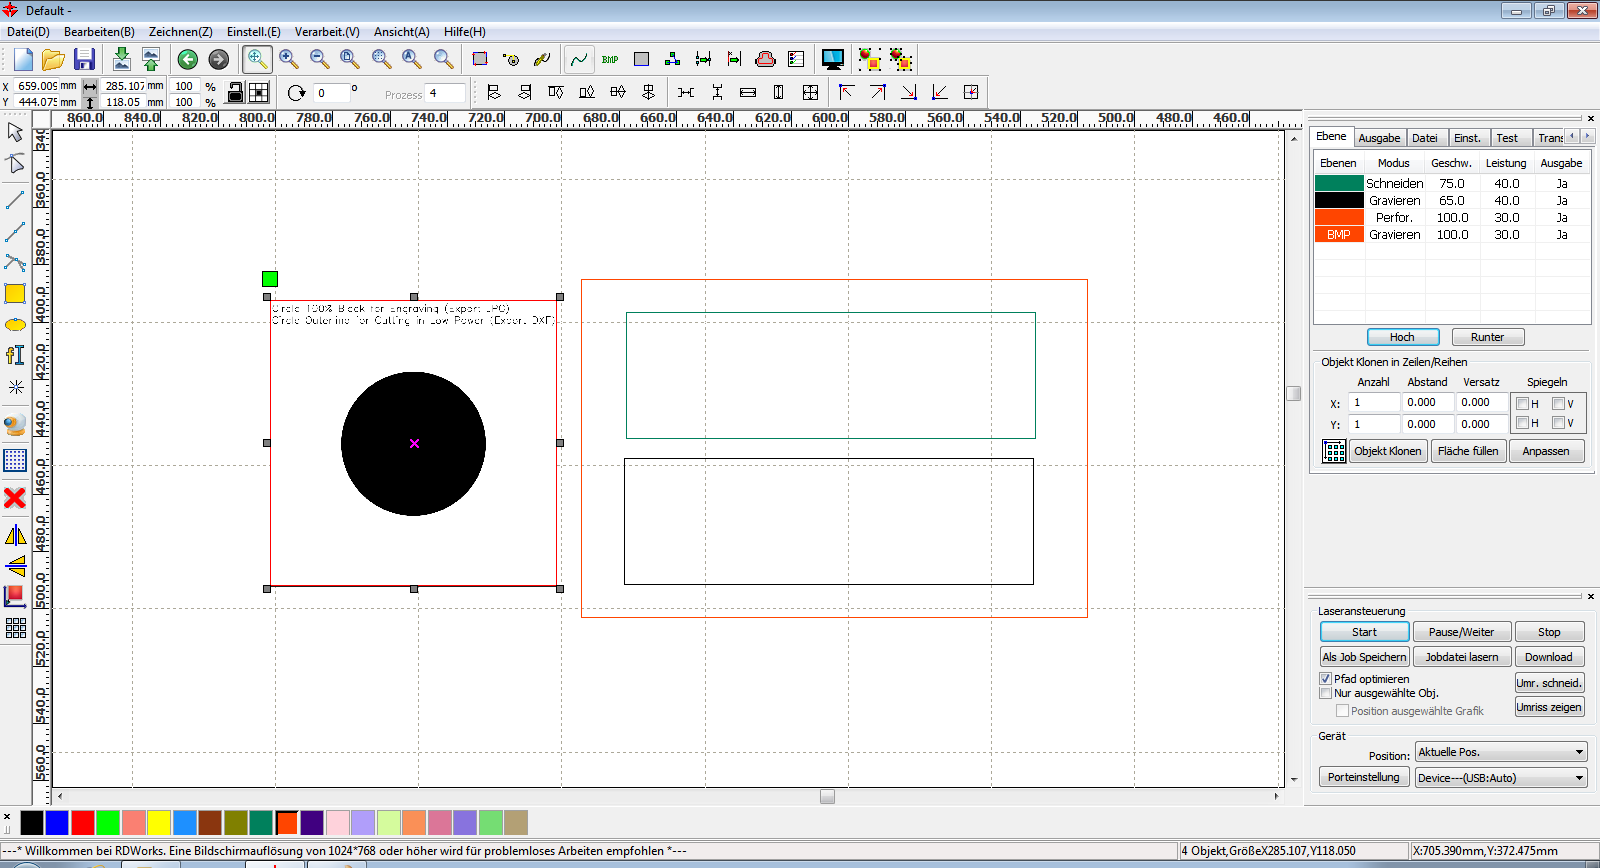
\includegraphics{assets/images/rdworks-software.PNG}
\caption{RDworks Software Oberfläche}\label{fig:rdsoftware}
}
\end{figure}

\newpage

\hypertarget{schneiden}{%
\paragraph{Schneiden}\label{schneiden}}

Um einen Schnitt einzurichten, kann mit einem Doppelklick auf die
entsprechende Ebene in der Ebenenpalette rechts oben (siehe
+@fig:rdsoftware) das Menü für die Einstellungen aufgerufen werden.
Siehe +@fig:rdcut. Hier kann eingestellt werden, wie schnell der
Laserkopf gefahren werden soll und mit welcher Intensität der Schnitt
stattfinden soll. Dazu muss:

\begin{enumerate}
\def\labelenumi{\arabic{enumi}.}
\tightlist
\item
  Die \texttt{Ausgabe} auf \texttt{Ja} stehen.
\item
  In \texttt{Geschw.(mm/s)} der gewünschte Wert eingetragen werden.
\item
  Der \texttt{Lasermodus} auf \texttt{Schneiden} stehen.
\item
  Im Feld mit der 1 und der Checkbox in \texttt{Min\ Leist\ (\%)} und
  \texttt{Max\ Leist.\ (\%)} der gleiche Wert eingetragen
  werden.\footnote{Die Software nutzt den Max Wert. Um Verwirrung zu
    vermeiden sollte jedoch in beide Felder der gleiche Wert eingetragen
    werden.}
\end{enumerate}

Alle weiteren Möglichkeiten sind zur Feineinstellung. Hierfür sollte das
Handbuch der Software zu Rate gezogen werden.

\begin{figure}
\hypertarget{fig:rdcut}{%
\centering
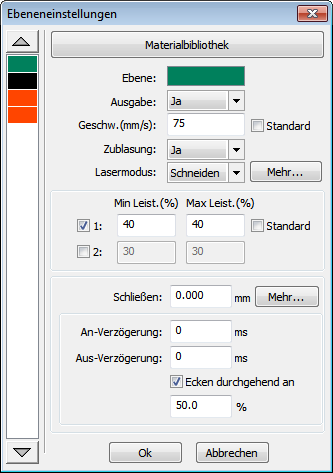
\includegraphics{assets/images/rdworks-schneiden.PNG}
\caption{RDWorks Ebeneneinstellungen Schneiden}\label{fig:rdcut}
}
\end{figure}

\hypertarget{gravieren}{%
\paragraph{Gravieren}\label{gravieren}}

Um eine Gravur einzurichten, kann mit einem Doppelklick auf die
entsprechende Ebene in der Ebenenpalette rechts oben (siehe
+@fig:rdsoftware) das Menü für die Einstellungen aufgerufen werden.
Siehe +@fig:rdgrav1. Hier können verschieden Parameter der Gravur
definiert werden. Dazu muss:

\begin{enumerate}
\def\labelenumi{\arabic{enumi}.}
\tightlist
\item
  Die \texttt{Ausgabe} auf \texttt{Ja} stehen.
\item
  In \texttt{Geschw.(mm/s)} der gewünschte Wert eingetragen werden.
\item
  Der \texttt{Lasermodus} auf \texttt{Gravur/Scan} stehen.
\item
  Das Feld \texttt{Graustufen\ ausgeb} gewählt sein oder nicht (siehe
  +@fig:rdgrav2).\footnote{Im Fall von Vektoren als Vorlage kann nur ein
    einheitlicher Wert gewählt werden. Das Feld ist dann nicht
    anwählbar.}
\item
  Die Leistung eingestellt werden

  \begin{enumerate}
  \def\labelenumii{\arabic{enumii}.}
  \tightlist
  \item
    Wenn einheitlich graviert werden soll, muss im Feld mit der 1 und
    der Checkbox in \texttt{Min\ Leist\ (\%)} und
    \texttt{Max\ Leist.\ (\%)} der gleiche Wert eingetragen
    werden.\footnote{Die Software nutzt den Max Wert. Um Verwirrung zu
      vermeiden sollte jedoch in beide Felder der gleiche Wert
      eingetragen werden.}. In diesem Fall sollte Graustufen ausgeben
    nicht gewählt sein.
  \item
    Wenn abhängig von den Graustufen des Bildes graviert werden soll.
    muss im Feld mit der 1 und der Checkbox in \texttt{Min\ Leist\ (\%)}
    die Leistung für das schwächste Grau eingetragen werden und im Feld
    \texttt{Max\ Leist.\ (\%)} die Leistung für das tiefste Schwarz
    eingetragen werden.\footnote{Aus Erfahrung hat sich ergeben, dass
      Werte unterhalb von 10\% Leistung kaum Ergebnis haben.}
  \end{enumerate}
\item
  Für den \texttt{Gravurmodus} gewählt werden ob\footnote{Die Gravurmodi
    bestimmen wie der Laser die Punkte abfährt. Zum Beispiel würde bei X
    beide Richtungen der Laser von Links anfahren, gravieren, auslaufen.
    Von Rechts wieder anfahren, gravieren, auslaufen und so weiter. Bei
    kleinen Schriften kann dieser Modus Treppen erzeugen. Es empfiehlt
    sich, wenn kleine Formen graviert werden sollen, den Laser nur aus
    einer Richtung gravieren zu lassen. Dadurch verdoppelt sich die
    Laufzeit für die Gravur.}

  \begin{enumerate}
  \def\labelenumii{\arabic{enumii}.}
  \tightlist
  \item
    X nur in eine Richtung graviert werden soll.
  \item
    X in beide Richtungen graviert werden soll.
  \item
    Y nur in eine Richtung graviert werden soll.
  \item
    Y in beide Richtungen graviert werden soll.
  \end{enumerate}
\item
  In \texttt{Zeilenabst.\ (mm)} der Abstand zwischen den einzelnen
  Gravurzeilen eingegeben werden. Der Standard ist 0,1mm. Dies kann aber
  noch weiter reduziert werden.
\end{enumerate}

Alle weiteren Möglichkeiten sind zur Feineinstellung. Hierfür sollte das
Handbuch der Software zu Rate gezogen werden.

\begin{figure}
\hypertarget{fig:rdgrav1}{%
\centering
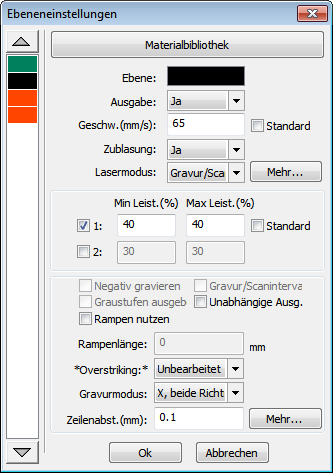
\includegraphics{assets/images/rdworks-gravieren1.PNG}
\caption{RDWorks Ebeneneinstellung Gravur Vektorform}\label{fig:rdgrav1}
}
\end{figure}

\begin{figure}
\hypertarget{fig:rdgrav2}{%
\centering
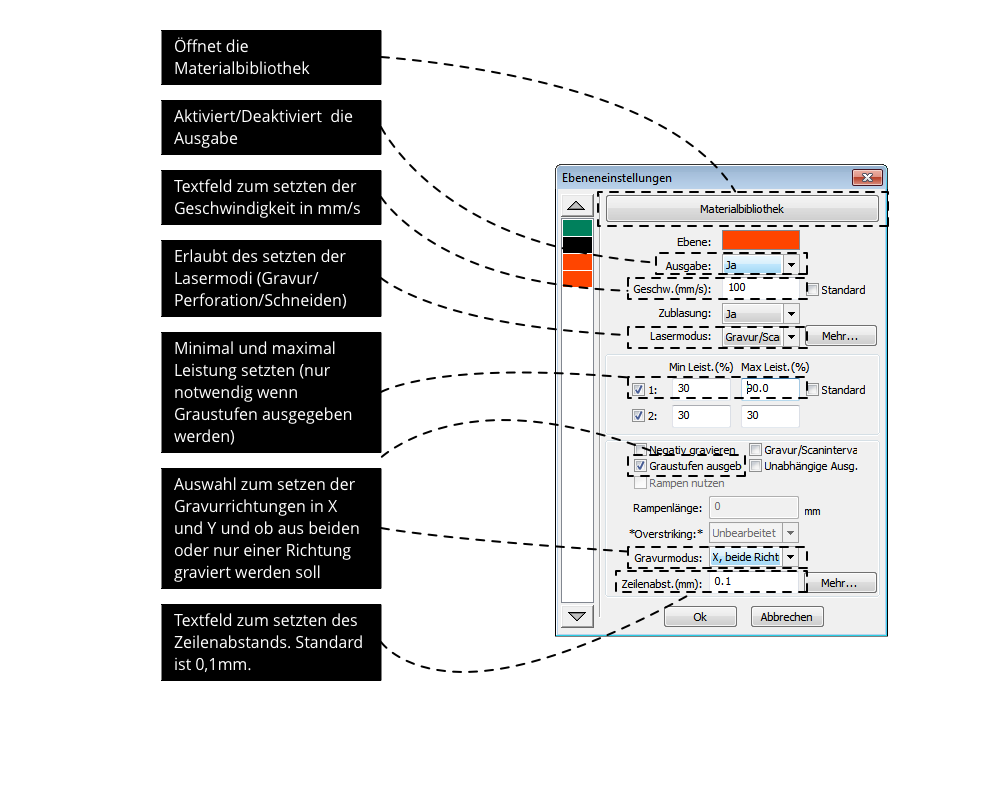
\includegraphics{assets/images/rdworks-gravur2.PNG}
\caption{RDWorks Ebeneneinstellung Gravur Vektorform}\label{fig:rdgrav2}
}
\end{figure}

\hypertarget{perforieren}{%
\paragraph{Perforieren}\label{perforieren}}

Um eine Perforation einzurichten kann mit einem Doppelklick auf die
entsprechende Ebene in der Ebenenpalette rechts oben (siehe
+@fig:rdsoftware) das Menü für die Einstellungen aufgerufen werden.
Siehe +@fig:rdperf. Hier kann eingestellt werden wie schnell der
Laserkopf gefahren werden soll, mit welcher Intensität die Perforation
stattfinden soll und wie das Verhältnis zwischen Schnitt -- Lücke --
Schnitt -- Lücke -- etc. sein soll. Dazu muss:

\begin{enumerate}
\def\labelenumi{\arabic{enumi}.}
\tightlist
\item
  Die \texttt{Ausgabe} auf \texttt{Ja} stehen.
\item
  In \texttt{Geschw.(mm/s)} der gewünschte Wert eingetragen werden.
\item
  Der \texttt{Lasermodus} auf \texttt{Schneiden} stehen.
\item
  Im Feld mit der 1 und der Checkbox in \texttt{Min\ Leist\ (\%)} und
  \texttt{Max\ Leist.\ (\%)} der gleiche Wert eingetragen
  werden.\footnote{Die Software nutzt den Max Wert. Um Verwirrung zu
    vermeiden sollte jedoch in beide Felder der gleiche Wert eingetragen
    werden.}
\item
  Das \texttt{Interval} auf einen mm Wert definiert werden.
\item
  Die \texttt{Punktlänge} auf einen mm Wert definiert werden.
\end{enumerate}

Alle weiteren Möglichkeiten sind zur Feineinstellung. Hierfür sollte das
Handbuch der Software zu Rate gezogen werden.

\begin{figure}
\hypertarget{fig:rdperf}{%
\centering
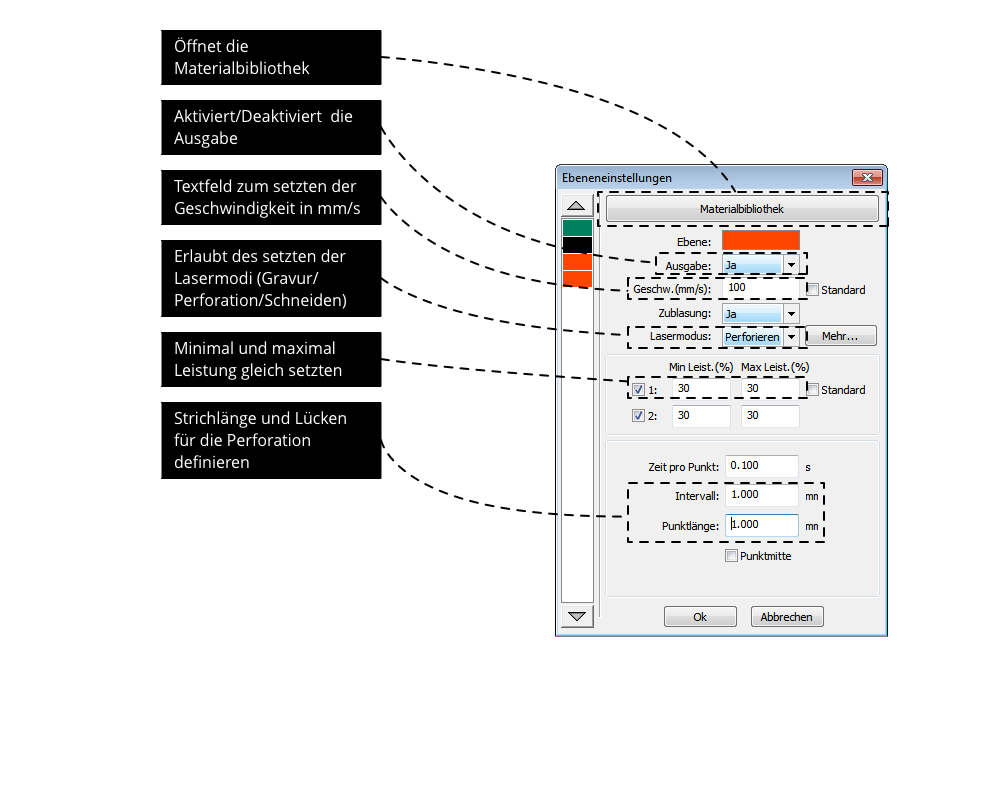
\includegraphics{assets/images/rdworks-perforieren.PNG}
\caption{RDWorks Ebeneneinstellungen Perforieren}\label{fig:rdperf}
}
\end{figure}

\hypertarget{material-bibliothek}{%
\subsubsection{Material Bibliothek}\label{material-bibliothek}}

Bei allen drei Arten von Jobs ist die Einstellung von Leistung und
Geschwindigkeit abhängig von dem Material. Glücklicherweise bietet die
Software bietet die Möglichkeit Einstellungen zu speichern. Diese können
in der Materialbibliothek abgelegt werden. Um diese zu öffnen muss mit
einem Doppelklick erst die Einstellung der Ebenen geöffnet werden. Im
oberen Bereich befindet sich ein Knopf (siehe zum Beispiel +@fig:rdperf)
für die Materialbibliothek (siehe +@fig:rdbib). Von dort aus können
Einstellungen geladen oder die aktuellen unter einem neuen Namen
gespeichert werden.\footnote{Wenn der Name bereits existiert, wird die
  alte Variante überschrieben.} Hierbei ist es ratsam einen
aussagekräftigen Namen zu wählen. Als Standard sollte folgendes Muster
gelten.

\begin{verbatim}
Material Stärke Jobtyp
\end{verbatim}

Dies würde bei einer Gravur auf einer 3mm Hochdichte Faserplatte (HDF)
zu \texttt{HDF\ 3mm\ Gravur} werden.

\begin{figure}
\hypertarget{fig:rdbib}{%
\centering
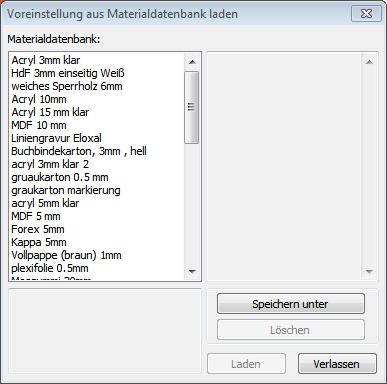
\includegraphics{assets/images/rdworks-materialbib.PNG}
\caption{RDworks Materialbibliothek}\label{fig:rdbib}
}
\end{figure}

\hypertarget{luxfcftung}{%
\subsubsection{Lüftung}\label{luxfcftung}}

\textbf{Achtung:} Das Aktivieren der Lüftung darf nicht vergessen
werden.

\hypertarget{den-job-starten}{%
\subsubsection{Den Job Starten}\label{den-job-starten}}

Wenn der Job in RDWorks soweit eingerichtet ist, wird es Zeit ihn zu
starten. Vorher sollte noch folgende Punkte ein letztes mal überprüft
werden.

\begin{enumerate}
\def\labelenumi{\arabic{enumi}.}
\tightlist
\item
  Ist der Fokus richtig gesetzt?
\item
  Steht der Laserkopf auf dem \texttt{Origin} (Null/Null) und ist der
  \texttt{Origin} richtig?
\item
  Ist die Lüftung aktiviert?
\item
  Ist die Abdeckung des Lasers geschlossen?
\item
  Passen die Daten auf das eingelegte Material?
\item
  Wurde die Zustimmungstaste gedrückt?
\end{enumerate}

\textbf{Zu 1):}

Es sollte ein letztes mal überlegt werden, ob der Fokus richtig gesetzt
wurde. Im Zweifelsfall sollte dieser Arbeitsschritt nochmal ausgeführt
werden.

\textbf{Zu 2):}

Der Laserkopf muss an seinem 0/0 Punkt stehen. Über einen Druck auf die
Taste \texttt{Esc} wird der Kopf auf seinen letzten \texttt{Origin}
zurückgesetzt.

\textbf{Zu 3):}

Die Lüftung muss aktiviert sein. Gerade bei Holz Materialien kann es zu
einer starken Rauchentwicklung kommen.

\textbf{Zu 4):}

Die Abdeckung des Lasers muss geschlossen sein, damit der Job gestartet
werden kann.

\textbf{Zu 5):}

Ob die Daten auf das Material passen, kann aus der Software heraus
überprüft werden. Rechts unten in RDWorks (siehe +@fig:rdsoftware) gibt
es die Möglichkeit, mit dem Knopf \texttt{Umriss\ zeigen} den Laserkopf
die äußeren Kanten der Vorlage abfahren zu lassen.

\textbf{Zu 6):}

Die Lasersteuerung weiß nicht, ob der Laser aktiviert ist oder nicht.
Daher kann ein Job gestartet werden, ohne das ein Schnitt, eine Gravur
oder eine Perforation zu Stande kommt. Um den Laser zu aktivieren muss:

\begin{enumerate}
\def\labelenumi{\arabic{enumi}.}
\tightlist
\item
  Die Abdeckung geschlossen sein.
\item
  Die Zustimmungstaste gedrückt werden (siehe +@fig:steuerung).
\end{enumerate}

Wenn all diese Maßnahmen getroffen wurden, kann über die Schaltfläche
\texttt{Start} (siehe +@fig:rdsoftware) in der Software der Job an den
Laser gesendet werden.

\hypertarget{der-job-luxe4uft}{%
\subsubsection{Der Job Läuft}\label{der-job-luxe4uft}}

Während ein Laser Job läuft darf die Anlage nicht unbeaufsichtigt
bleiben. Ebenfalls sollte die Abdeckung nicht geöffnet werden. Falls es
nötig ist die Abdeckung zu öffnen, wird der Job pausiert. Falls ab dem
aktuellen Punkt weiter gelasert werden soll, kann dies über die
\texttt{Start/Pause} (siehe +@fig:steuerung) Taste veranlasst werden.
Dabei ist drauf zu achten, dass nochmals die \texttt{Zustimmungstaste}
gedrückt werden muss. Sonst fährt der Laserkopf weiter, aber der Laser
wird nicht wieder aktiviert.

\hypertarget{abschaltung}{%
\subsection{Abschaltung}\label{abschaltung}}

Der Prozess der Abschaltung ist grundsätzlich die umgekehrte Variante
der Inbetriebnahme bis auf einige Ausnahmen.

\hypertarget{laserkopf-in-ausgangspostion}{%
\subsubsection{Laserkopf in
Ausgangspostion}\label{laserkopf-in-ausgangspostion}}

Da der Laser nach dem Anschalten sofort eine Referenzfahrt macht, muss
vor dem Abschalten der Laserkopf in die rechte obere Ecke der
Arbeitsfläche gefahren werden und dort seinen letzten \texttt{Origin}
erhalten. Damit kann verhindert werden, dass die/der nächste Nutzer/in
den Laserkopf beschädigt, weil Material auf der Arbeitsfläche vergessen
wurde oder das Gitter dem Distanztaster im Weg ist.

\hypertarget{z-achse-runter-fahren}{%
\subsubsection{Z-Achse Runter Fahren}\label{z-achse-runter-fahren}}

Um die Inbetriebnahme weiter zu vereinfachen, sollte die Z-Achse ein
Stück runter gefahren werden. Nicht so weit, dass das Gitter unter den
Absatz rutschen kann. Jedoch so weit, dass optisch direkt sichtbar ist,
dass der Taster nicht gegen das Gitter stoßen kann.

\hypertarget{abschaltung-steuerung-und-laser}{%
\subsubsection{Abschaltung Steuerung und
Laser}\label{abschaltung-steuerung-und-laser}}

Ist der Laserkopf in der Ausgangsposition und der \texttt{Origin} wurde
gesetzt, kann mit der Laser auf \texttt{Aus} gestellt werden und die
Steuerung ebenfalls (siehe +@fig:steuerung).

\hypertarget{abschaltung-hauptstrom}{%
\subsubsection{Abschaltung Hauptstrom}\label{abschaltung-hauptstrom}}

Nach dem letzten Setzten der Ausgangsposition, der Anpassung der Z-Achse
und dem Abschalten der Anlage, kann der Hauptstrom abgeschaltet werden
(siehe +@fig:hauptschalter).

\hypertarget{luxfcftung-1}{%
\subsubsection{Lüftung}\label{luxfcftung-1}}

Jetzt kann die Lüftung in Bereich 1 (siehe +@fig:luefter) ausgeschaltet
werden.

\hypertarget{oberlicht-schlieuxdfen}{%
\subsubsection{Oberlicht Schließen}\label{oberlicht-schlieuxdfen}}

Zuletzt wird das Oberlicht, an dem die Lüftung hängt, geschlossen.

\hypertarget{materialien}{%
\subsection{Materialien}\label{materialien}}

\textbf{In dem Laser dürfen keine PVC-haltigen Materialien geschnitten
werden!} PVC-haltige Material erzeugen Chlorwasserstoffgase, die höchst
giftig sind und auch die Maschine angreifen. Wenn es nötig ist, Polymere
zu identifizieren, kann
\href{http://www.chymist.com/Polymer\%20Identification.pdf}{dieses
Paper} ("Identification Of Polymers") von David A. Katz ebenfalls zu
Rate gezogen werden.

Das FabLab München hat in seinem Wiki eine
\href{http://wiki.fablab-muenchen.de/pages/viewpage.action?pageId=1179992}{umfassende
Liste} von möglichen und unmöglichen Materialien und das Wiki des
\href{http://atxhackerspace.org/wiki/Laser_Cutter_Materials}{ATX
Hackerspace} ist ebenfalls eine gute Quelle.

\begin{quote}
\textbf{Schneidbare Materialien:}

\begin{itemize}
\tightlist
\item
  Holz (bis ca. 6mm Dicke)
\item
  Papier
\item
  Karton/Pappe
\item
  Acryl/Plexiglas (bis ca. 6mm Dicke) bzw.
  PMMA~\href{https://de.wikipedia.org/wiki/Polymethylmethacrylat}{(Polymethylmethacrylat)}
\item
  Stoffe
\item
  Leder
\item
  Linoleum
\item
  Pertinax
\item
  Schleifpapier (von der Rückseite her)
\item
  Elfenbein / Horn
\item
  Seide
\item
  Delrin (POM, acetal)
\item
  Mylar (polyester)
\item
  PETG (polyethylene terephthalate glycol)
\end{itemize}

Gravierbar sind dieselben Materialien plus:

\begin{itemize}
\tightlist
\item
  lackierte Metalle
\item
  Edelstahl (mit speziellem Sprüh-Lack)
\item
  eloxiertes Alu
\item
  Glas
\item
  Stein (beschränkt)
\item
  Marmor (beschränkt)
\item
  Gips
\item
  Fleece
\end{itemize}

\textbf{Auf keinen Fall dürfen geschnitten werden:}

\begin{itemize}
\tightlist
\item
  PVC/Vinyl, Neopren und sämtliche andere chlorhaltigen Stoffe!
  Entwickelt giftige Dämpfe! Außerdem geht die Maschine kaputt.
\item
  hoch entzündliche/explosive Materialien (versteht sich von selbst)
\item
  ABS (acrylonitrile butadiene styrene) - stinkt gewaltig und erzeugt
  giftige Gase
\item
  halogenierten Monomeren bestehende Kunststoffe wie~, Vinyl,
  Polydibromstyrol,~~(Teflon)
\item
  Bakelit -~Bitte nicht lasern
  -~\href{http://www.baubegriffe.com/Bausachverstandiger_Holzmann-Bauberatung/Blog/Eintrage/2011/10/11_122_Schadstoffe_die_unser_Leben_beeinflussen.html}{siehe
  Link}
\end{itemize}

Funktioniert nicht gut, besser nicht verwenden:

\begin{itemize}
\tightlist
\item
  Polykarbonat (PC, Lexan) -- schlechter Schnitt, verfärbt sich, fängt
  Feuer
\item
  High density polyethylene (HDPE) -- schmilzt
\item
  Polypropylene (PP) -- schmilzt (dünne Folien bis 1mm OK)
\item
  Polystyrol (PS) -- schmilzt (dünne Platten OK)
\item
  Polyethylene (PE) -- schmilzt
\item
  Styrodur -- schmilzt
\item
  Nylon -- schmilzt
\item
  Moosgummi~--~Würde ich nicht empfehlen, wenn Benzol zum Aufschäumen
  verwendet
  wurde~~-~\href{http://www.baubegriffe.com/Bausachverstandiger_Holzmann-Bauberatung/Blog/Eintrage/2011/10/11_122_Schadstoffe_die_unser_Leben_beeinflussen.html}{siehe
  Link}
\item
  Schellack --~~auch hier ist die Beschaffenheit der Politur bzw der
  Beschichtung zu wissen, im Zweifel eher nicht.
\item
  Kapton tape (Polyamide) - muss nachgefragt werden
  -~\href{http://www.potomac-laser.com/services/applications/laser-micromachining-of-dupont-kapton-polyimide/}{siehe
  Link}
\end{itemize}

\textbf{Materialien die unser Laser nicht schneiden kann:}

\begin{itemize}
\tightlist
\item
  Metalle aller Art
\item
  Kohlefaser
\item
  Glas
\item
  Fiberglas
\item
  Platinen
\end{itemize}

\href{http://wiki.fablab-muenchen.de/pages/viewpage.action?pageId=1179992}{Quelle}
\end{quote}

\hypertarget{zugang-zu-anlage-schluxfcssel-und-computer}{%
\subsection{Zugang zu Anlage, Schlüssel und
Computer}\label{zugang-zu-anlage-schluxfcssel-und-computer}}

Der Zugang zur Anlage wird über
\href{https://docs.google.com/spreadsheets/d/1I4rYd23biIntc6wfrVsdPKd0qprd70GNY0aXA4jAOJA/edit\#gid=0}{dieses
Google Doc} geregelt.\footnote{Achtung die Adresse des Google Docs
  könnte sich ändern.} Dort sind alle Personen eingetragen, die sich am
Informationsstand im Hauptgebäude gegen Unterschrift den Schlüsselbund
abholen dürfen. An diesem Bund ist:

\begin{itemize}
\tightlist
\item
  ein Schlüssel für die Steuerung
\item
  ein Schlüssel für den Laser
\item
  ein Schlüssel für Spind Nummer 01
\item
  ein Dongel für LW 022
\end{itemize}

Um die Zugangsberechtigung zu erwerben muss:

\begin{itemize}
\tightlist
\item
  eine Einweisung an der Anlage stattgefunden haben.
\item
  eine Abnahme durch die Administratoren stattgefunden haben.
\item
  die jährliche Sicherheitseinweisung der Modellbauwerkstätten besucht
  worden sein.
\item
  die Werkstattordnung gelesen und gegengezeichnet worden sein.
\end{itemize}

Wir behalten uns vor die Berechtigung nach einem derzeit noch
unbestimmten Zeitraum wieder zu entziehen, da bei nicht Nutzung der
Anlage auch die Routine verloren geht.

\hypertarget{der-computer}{%
\subsubsection{Der Computer}\label{der-computer}}

Die FHP stellt seinen Studierenden einen Computer zur Verfügung. Auf
diesem Computer ist nur die Software RDWorks und
\href{https://inkscape.org/en/}{Inkscape} installiert. Da das
Betriebssystem veraltet ist, sollte davon abgesehen werden, diesen
Rechner an das Internet anzuschließen. Daten müssen per USB Stick
übertragen werden. Die FHP führt keine Backups dieses Rechners aus und
behält sich vor alle dort abgelegten Daten zu löschen, falls es
notwendig sein sollte. Es existiert eine Partition \texttt{E\ (Daten)},
auf der eigene Ordner angelegt werden dürfen.

\hypertarget{terminvergabe}{%
\subsection{Terminvergabe}\label{terminvergabe}}

Die Terminvergabe läuft über die Terminfunktion des Incom.org Workspaces
\href{https://fhp.incom.community/workspace/6508}{Laser KNLG Base · FHP}
und nach dem „First Come First Serverd`` Prinzip. Termine sind bindend
und müssen dort vorab eingestellt werden. Wenn Termine nicht
wahrgenommen werden können, müssen sie dort auch wieder gelöscht werden.
Mehr als 2 Termine an einem Tag ist aus Erfahrungswerten kaum zu
handhaben.

\hypertarget{checklist}{%
\subsection{Checklist}\label{checklist}}

Es folgt eine Checkliste für den gesamten Betriebsprozess. Sie sollte
ausgedruckt und als Referenz griffbereit sein.

\textbf{Inbetriebnahme}

\begin{itemize}
\tightlist
\item[$\square$]
  Hauptstrom anschalten
\item[$\square$]
  Abdeckung öffnen\\
\item[$\square$]
  Arbeitsfläche leeren\\
\item[$\square$]
  Laserkopf höher als das Gitter?\\
\item[$\square$]
  Gitter nicht unter dem Absatz?\\
\item[$\square$]
  Distanztaster ist nicht verrußt?\\
\item[$\square$]
  Distanztaster bewegt sich leicht und verkantet nicht?\\
\item[$\square$]
  Hand über den Notaus!\\
\item[$\square$]
  Steuerung mit Schlüssel anschalten\\
\item[$\square$]
  Laserkopf beobachten bis die Referenzfahrt vorbei ist\\
\item[$\square$]
  Laser mit dem Schlüssel anschalten
\end{itemize}

\textbf{Laser Job}

\begin{itemize}
\tightlist
\item[$\square$]
  Daten einrichten\\
\item[$\square$]
  Autofokus setzten. Der Distanztaster ist relevant nicht der
  Laserpunkt!\\
\item[$\square$]
  Material final positionieren\\
\item[$\square$]
  Origin setzten\\
\item[$\square$]
  Passt die Vorlage auf das Material? Umrisse zeigen.
\item[$\square$]
  Oberlicht öffnen\\
\item[$\square$]
  Lüftung anschalten
\item[$\square$]
  Abdeckung schließen\\
\item[$\square$]
  Zustimmungstaste drücken\\
\item[$\square$]
  In der Software \texttt{Start} drücken\\
\item[$\square$]
  Laser beobachten (im Falle eines Feuers Ruhe bewahren)
\end{itemize}

\textbf{Feuer}

\begin{itemize}
\tightlist
\item[$\square$]
  Abdeckung NICHT öffnen\\
\item[$\square$]
  Laserjob stoppen\\
\item[$\square$]
  Lüftung abschalten\\
\item[$\square$]
  Feuerlöscher verwenden\\
\item[$\square$]
  Feuerwehr rufen
\end{itemize}

\textbf{Abschaltung}

\begin{itemize}
\tightlist
\item[$\square$]
  Arbeitsfläche frei räumen\\
\item[$\square$]
  Kleine Materialreste entfernen\\
\item[$\square$]
  Laserkopf in die rechte obere Ecke fahren\\
\item[$\square$]
  Origin dort setzten\\
\item[$\square$]
  Z-Achse runter fahren\\
\item[$\square$]
  Z-Achse nicht tiefer als den Absatz fahren\\
\item[$\square$]
  Maschine reinigen\\
\item[$\square$]
  Laser abschalten\\
\item[$\square$]
  Steuerung abschalten\\
\item[$\square$]
  Hauptstrom abschalten\\
\item[$\square$]
  Abdeckung schließen\\
\item[$\square$]
  Lüftung abschalten\\
\item[$\square$]
  Oberlicht schließen\\
\item[$\square$]
  Computer und Kiste zurück in Spind Nummer 01\\
\item[$\square$]
  Werkstatt verriegeln\\
\item[$\square$]
  Schlüssel beim Pförtner abgeben
\end{itemize}

\textbf{Reinignug}

\begin{itemize}
\tightlist
\item[$\square$]
  Reste entfernen
\item[$\square$]
  Taster reinigen
\item[$\square$]
  Innenraum aussaugen
\end{itemize}

\hypertarget{hersteller-sabko}{%
\subsection{Hersteller Sabko}\label{hersteller-sabko}}

Sabko-GmbH\\
AG Wittlich -HRB 42278\\
UST-IdNr. DE286904964\\
vertreten durch die Geschäftsführer:\\
Sabine Lunkes, Kauffrau\\
Konrad Kraus, Mechatronikmeister

Kiemstrasse 10\\
54311 Trierweiler - Industriegebiet\\
Tel. 0049 (0) 651-88094\\
E-Mail:
\href{mailto:info@sabko-gmbh.com}{\nolinkurl{info@sabko-gmbh.com}}

\hypertarget{uxfcber-dieses-dokument}{%
\subsection{Über dieses Dokument}\label{uxfcber-dieses-dokument}}

Die aktuellste Version dieses Dokuments kann immer auf
\href{https://github.com/FH-Potsdam/the-ultimate-laser-guide/raw/master/The-Ultimate-Laser-Guide.pdf}{GitHub
runter geladen} werden. Anregungen, Erweiterungen und Fehlerkorrekturen
sind sehr gerne gesehen.

\begin{itemize}
\tightlist
\item
  Korrekturen als Kommentare im PDF oder als
  \href{https://github.com/FH-Potsdam/the-ultimate-laser-guide/issues}{Issue}
  auf GitHub
\item
  Ganze Kapitel bitte als reinen Text ohne Formatierungen
\item
  Das alles natürlich auch gerne als Pull Request auf GitHub
\end{itemize}

\hypertarget{schriften}{%
\subsubsection{Schriften}\label{schriften}}

Es werden die Schriften \href{https://github.com/IBM/plex}{IBM Plex}
Sans und Mono genutzt. Sollte Pandoc diese nicht erkennen, müssen diese
installiert und aktiviert sein. Es reicht dann nicht die Schrift Dateien
im Benutzer Ordner \texttt{/Users/you/Library/Fonts/} zu haben. Auf dem
System auf dem dieses PDF generiert wurde mussten diese unter
\texttt{/Library/Fonts/} installiert sein.

\hypertarget{dokument-generieren}{%
\subsubsection{Dokument Generieren}\label{dokument-generieren}}

Das Dokument ist überwiegend in Pandoc Markdown \texttt{{[}M↓{]}}
geschrieben.\footnote{Es wurden wenige \LaTeX  Befehle verwendet für ein
  besseres Layout.} Dort wo \texttt{{[}M↓{]}} nicht mehr weiter kommt
wurde \LaTeX genutzt. Um das finale PDF zu generieren muss
\href{https://pandoc.org/}{Pandoc} mit dem dem
\href{https://github.com/tomduck/pandoc-fignos}{fignos} Filter
installiert sein. Um die Ausführung zu vereinfachen wurde das
entsprechende Shell Befehl in ein npm script gespeichert.

\hypertarget{mac}{%
\paragraph{Mac}\label{mac}}

\begin{verbatim}
    brew cask install mactex
    brew install node
    brew install pandoc
    pip install pandoc-fignos
    git clone git@github.com:FH-Potsdam/the-ultimate-laser-guide.git
    cd ./the-ultimate-laser-guide
    npm install
    npm run pandoc
\end{verbatim}

\hypertarget{linux}{%
\paragraph{Linux}\label{linux}}

Requirements: NodeJS \& Python

\begin{verbatim}
sudo apt-get update
sudo apt-get install pandoc
sudo apt-get isntall texlive
pip[3] install pandoc-fignos
\end{verbatim}

\hypertarget{lizenz}{%
\subsection{Lizenz}\label{lizenz}}

Dieses Dokument und alle Bilder, soweit nicht anders gekennzeichnet,
sind unter MIT Lizenz.

Copyright (c) 2017 Fabian Morón Zirfas \& Fachhochschule Potsdam

DE:

Hiermit wird unentgeltlich jeder Person, die eine Kopie der Software und
der zugehörigen Dokumentationen (die "Software") erhält, die Erlaubnis
erteilt, sie uneingeschränkt zu nutzen, inklusive und ohne Ausnahme mit
dem Recht, sie zu verwenden, zu kopieren, zu verändern, zusammenzufügen,
zu veröffentlichen, zu verbreiten, zu unterlizenzieren und/oder zu
verkaufen, und Personen, denen diese Software überlassen wird, diese
Rechte zu verschaffen, unter den folgenden Bedingungen:

Der obige Urheberrechtsvermerk und dieser Erlaubnisvermerk sind in allen
Kopien oder Teilkopien der Software beizulegen.

DIE SOFTWARE WIRD OHNE JEDE AUSDRÜCKLICHE ODER IMPLIZIERTE GARANTIE
BEREITGESTELLT, EINSCHLIESSLICH DER GARANTIE ZUR BENUTZUNG FÜR DEN
VORGESEHENEN ODER EINEM BESTIMMTEN ZWECK SOWIE JEGLICHER
RECHTSVERLETZUNG, JEDOCH NICHT DARAUF BESCHRÄNKT. IN KEINEM FALL SIND
DIE AUTOREN ODER COPYRIGHTINHABER FÜR JEGLICHEN SCHADEN ODER SONSTIGE
ANSPRÜCHE HAFTBAR ZU MACHEN, OB INFOLGE DER ERFÜLLUNG EINES VERTRAGES,
EINES DELIKTES ODER ANDERS IM ZUSAMMENHANG MIT DER SOFTWARE ODER
SONSTIGER VERWENDUNG DER SOFTWARE ENTSTANDEN.

EN:

Permission is hereby granted, free of charge, to any person obtaining a
copy of this software and associated documentation files (the
"Software"), to deal in the Software without restriction, including
without limitation the rights to use, copy, modify, merge, publish,
distribute, sublicense, and/or sell copies of the Software, and to
permit persons to whom the Software is furnished to do so, subject to
the following conditions:

The above copyright notice and this permission notice shall be included
in all copies or substantial portions of the Software.

THE SOFTWARE IS PROVIDED "AS IS", WITHOUT WARRANTY OF ANY KIND, EXPRESS
OR IMPLIED, INCLUDING BUT NOT LIMITED TO THE WARRANTIES OF
MERCHANTABILITY, FITNESS FOR A PARTICULAR PURPOSE AND NONINFRINGEMENT.
IN NO EVENT SHALL THE AUTHORS OR COPYRIGHT HOLDERS BE LIABLE FOR ANY
CLAIM, DAMAGES OR OTHER LIABILITY, WHETHER IN AN ACTION OF CONTRACT,
TORT OR OTHERWISE, ARISING FROM, OUT OF OR IN CONNECTION WITH THE
SOFTWARE OR THE USE OR OTHER DEALINGS IN THE SOFTWARE.

\end{document}
